% From https://github.com/UWIT-IAM/UWThesis
\documentclass[print]{nuthesis}
\usepackage{amssymb, amsthm, amsmath, amsfonts}
\usepackage{wasysym}
\usepackage{mathrsfs}
% \usepackage{hyperref}
\usepackage{graphicx}
\usepackage{lineno}
\usepackage[colorinlistoftodos]{todonotes}
\usepackage{listings}
%\usepackage{breqn}
\usepackage{cancel, enumerate}
\usepackage{rotating, environ}
\usepackage{caption}
\usepackage{subcaption}
\usepackage[inline]{enumitem}
\usepackage{dirtree}

\newtheorem{thm}{Theorem}
\newtheorem{defn}{Definition}
\newtheorem{prop}{Proposition}
\newtheorem{lemma}{Lemma}
\newtheorem{cor}{Corollary}

% Syntax highlighting #22
  \usepackage{color}
  \usepackage{fancyvrb}
  \newcommand{\VerbBar}{|}
  \newcommand{\VERB}{\Verb[commandchars=\\\{\}]}
  \DefineVerbatimEnvironment{Highlighting}{Verbatim}{commandchars=\\\{\}}
  % Add ',fontsize=\small' for more characters per line
  \usepackage{framed}
  \definecolor{shadecolor}{RGB}{248,248,248}
  \newenvironment{Shaded}{\begin{snugshade}}{\end{snugshade}}
  \newcommand{\AlertTok}[1]{\textcolor[rgb]{0.94,0.16,0.16}{#1}}
  \newcommand{\AnnotationTok}[1]{\textcolor[rgb]{0.56,0.35,0.01}{\textbf{\textit{#1}}}}
  \newcommand{\AttributeTok}[1]{\textcolor[rgb]{0.77,0.63,0.00}{#1}}
  \newcommand{\BaseNTok}[1]{\textcolor[rgb]{0.00,0.00,0.81}{#1}}
  \newcommand{\BuiltInTok}[1]{#1}
  \newcommand{\CharTok}[1]{\textcolor[rgb]{0.31,0.60,0.02}{#1}}
  \newcommand{\CommentTok}[1]{\textcolor[rgb]{0.56,0.35,0.01}{\textit{#1}}}
  \newcommand{\CommentVarTok}[1]{\textcolor[rgb]{0.56,0.35,0.01}{\textbf{\textit{#1}}}}
  \newcommand{\ConstantTok}[1]{\textcolor[rgb]{0.00,0.00,0.00}{#1}}
  \newcommand{\ControlFlowTok}[1]{\textcolor[rgb]{0.13,0.29,0.53}{\textbf{#1}}}
  \newcommand{\DataTypeTok}[1]{\textcolor[rgb]{0.13,0.29,0.53}{#1}}
  \newcommand{\DecValTok}[1]{\textcolor[rgb]{0.00,0.00,0.81}{#1}}
  \newcommand{\DocumentationTok}[1]{\textcolor[rgb]{0.56,0.35,0.01}{\textbf{\textit{#1}}}}
  \newcommand{\ErrorTok}[1]{\textcolor[rgb]{0.64,0.00,0.00}{\textbf{#1}}}
  \newcommand{\ExtensionTok}[1]{#1}
  \newcommand{\FloatTok}[1]{\textcolor[rgb]{0.00,0.00,0.81}{#1}}
  \newcommand{\FunctionTok}[1]{\textcolor[rgb]{0.00,0.00,0.00}{#1}}
  \newcommand{\ImportTok}[1]{#1}
  \newcommand{\InformationTok}[1]{\textcolor[rgb]{0.56,0.35,0.01}{\textbf{\textit{#1}}}}
  \newcommand{\KeywordTok}[1]{\textcolor[rgb]{0.13,0.29,0.53}{\textbf{#1}}}
  \newcommand{\NormalTok}[1]{#1}
  \newcommand{\OperatorTok}[1]{\textcolor[rgb]{0.81,0.36,0.00}{\textbf{#1}}}
  \newcommand{\OtherTok}[1]{\textcolor[rgb]{0.56,0.35,0.01}{#1}}
  \newcommand{\PreprocessorTok}[1]{\textcolor[rgb]{0.56,0.35,0.01}{\textit{#1}}}
  \newcommand{\RegionMarkerTok}[1]{#1}
  \newcommand{\SpecialCharTok}[1]{\textcolor[rgb]{0.00,0.00,0.00}{#1}}
  \newcommand{\SpecialStringTok}[1]{\textcolor[rgb]{0.31,0.60,0.02}{#1}}
  \newcommand{\StringTok}[1]{\textcolor[rgb]{0.31,0.60,0.02}{#1}}
  \newcommand{\VariableTok}[1]{\textcolor[rgb]{0.00,0.00,0.00}{#1}}
  \newcommand{\VerbatimStringTok}[1]{\textcolor[rgb]{0.31,0.60,0.02}{#1}}
  \newcommand{\WarningTok}[1]{\textcolor[rgb]{0.56,0.35,0.01}{\textbf{\textit{#1}}}}

%% https://github.com/rstudio/rmarkdown/issues/1649
\newlength{\cslhangindent}
\setlength{\cslhangindent}{1.5em}
\newenvironment{CSLReferences}[2]%
{\setlength{\parindent}{0pt}%
\everypar{\setlength{\hangindent}{\cslhangindent}}\ignorespaces}%
{\par}

% fix for pandoc 1.14
\providecommand{\tightlist}{%
  \setlength{\itemsep}{0pt}\setlength{\parskip}{0pt}}

%% something about tables, from https://github.com/ismayc/thesisdown/issues/122
\usepackage{calc}

%% for copyright symbol
\usepackage{textcomp}

%% to allow to rotate pages to landscape
\usepackage{lscape}
%% to adjust table column width
\usepackage{tabularx}

% suppress bottom page numbers on first page of each chapter
% because they overlap with text
\usepackage{etoolbox}
\patchcmd{\chapter}{plain}{empty}{}{}

%% for more attractive tables
\usepackage{booktabs}
\usepackage{longtable}


\usepackage{graphicx}


% Double spacing, if you want it.
\def\dsp{\def\baselinestretch{2.0}\large\normalsize}
% \dsp

% If the Grad. Division insists that the first paragraph of a section
% be indented (like the others), then include this line:
\usepackage{indentfirst}

%%%%%%%%%%%%%%%%%%
% If you want to use "sections" to partition your thesis
% un-comment the following:
%
% \counterwithout{section}{chapter}
% \setsecnumdepth{subsubsection}
% \def\sectionmark#1{\markboth{#1}{#1}}
% \def\subsectionmark#1{\markboth{#1}{#1}}
% \renewcommand{\thesection}{\arabic{section}}
% \renewcommand{\thesubsection}{\thesection.\arabic{subsection}}
% \makeatletter
% \let\l@subsection\l@section
% \let\l@section\l@chapter
% \makeatother

\renewcommand{\thetable}{\arabic{table}}
\renewcommand{\thefigure}{\arabic{figure}}

%%%%%%%%%%%%%%%%%%


%% Stuff from https://github.com/suchow/Dissertate

% The following line would print the thesis in a postscript font

% \usepackage{natbib}
% \def\bibpreamble{\protect\addcontentsline{toc}{chapter}{Bibliography}}

\setcounter{tocdepth}{1} % Print the chapter and sections to the toc
% controls depth of table of contents (toc): 0 = chapter, 1 = section, 2 = subsection

\usepackage{natbib}


% commands and environments needed by pandoc snippets
% extracted from the output of `pandoc -s`
%% Make R markdown code chunks work
\usepackage{array}
\usepackage{amssymb,amsmath}
\usepackage{ifxetex,ifluatex}
\ifxetex
  \usepackage{fontspec,xltxtra,xunicode}
  \defaultfontfeatures{Mapping=tex-text,Scale=MatchLowercase}
\else
  \ifluatex
    \usepackage{fontspec}
    \defaultfontfeatures{Mapping=tex-text,Scale=MatchLowercase}
  \else
    \usepackage[utf8]{inputenc}
  \fi
\fi
\usepackage{color}
\usepackage{fancyvrb}


\ifxetex
  \usepackage[setpagesize=false, % page size defined by xetex
              unicode=false, % unicode breaks when used with xetex
              xetex,
              colorlinks=true,
              linkcolor=blue]{hyperref}
\else
  \usepackage[unicode=true,
              colorlinks=true,
              linkcolor=blue]{hyperref}
\fi
\hypersetup{breaklinks=true, pdfborder={0 0 0}}
\setlength{\parindent}{20pt}
\setlength{\parskip}{6pt plus 2pt minus 1pt}
\setlength{\emergencystretch}{3em}  % prevent overfull lines
\setcounter{secnumdepth}{2} %% controls section numbering, e.g. 1 or 1.2, or 1.2.3



%  ----  Text Colors  ------------------------------------------
%
% Assign colors to writers for review
%
\newcommand{\db}[1]{{\textcolor{blue}{#1}}}
\newcommand{\svp}[1]{{\textcolor{RedOrange}{#1}}}
\newcommand{\cochaircol}[1]{{\textcolor{Green}{#1}}}
%


%  --- Code chunk font size -----------------------------------------------
% https://stackoverflow.com/questions/38323331/code-chunk-font-size-in-beamer-with-knitr-and-latexhttps://stackoverflow.com/questions/38323331/code-chunk-font-size-in-beamer-with-knitr-and-latex

%% change fontsize of R code
\let\oldShaded\Shaded
\let\endoldShaded\endShaded
\renewenvironment{Shaded}{\footnotesize\oldShaded}{\endoldShaded}

%% change fontsize of output
\let\oldverbatim\verbatim
\let\endoldverbatim\endverbatim
\renewenvironment{verbatim}{\footnotesize\oldverbatim}{\endoldverbatim}


\begin{document}
% \linenumbers{}
%% Start formatting the first few special pages
%% frontmatter is needed to set the page numbering correctly
\frontmatter
%% from thesisdown
% To pass between YAML and LaTeX the dollar signs are added by CII
\title{DATA SCIENCE, DASHBOARDS, AND THE WAY IT WORKS WITH STATISTICS}
\author{Denise Renee Bradford}
\adviser{Susan R. VanderPlas, Ph.D}
% \adviserAbstract{}
\major{Statistics}
\degreemonth{Month}
\degreeyear{Year}
% \copyrightpage
%%
%% For most people the defaults will be correct, so they are commented
%% out. To manually set these, just uncomment and make the needed
%% changes.
%% \college{Your college}
%% \city{Your City}
%%
%% For most people the following can be changed with a class
%% option. To manually set these, just uncomment the following and
%% make the needed changes.
%% \doctype{Thesis or Dissertation}
%% \degree{Your degree}
%% \degreeabbreviation{Your degree abbr.}
%%
%% Now that we know everything we need, we can generate the title page
%% itself.
%%
\maketitle


\begin{abstract}
    Here is my abstract. \emph{(350 word limit)}
\end{abstract}

%% Optional
\begin{copyrightpage}
\end{copyrightpage}

%% Optional
\begin{dedication}
Dedicated to\ldots{}
\end{dedication}

%%%%%%%%%%%%%%%%%%%
% Acknowledgments
%%%%%%%%%%%%%%%%%%%
\begin{acknowledgments}
Thank you to all my people!
\end{acknowledgments}
%%%%%%%%%%%%%%%%%%%

%%%%%%%%%%%%%%%%%%%
% Grant Information
%%%%%%%%%%%%%%%%%%%
% \begin{grantinfo}
%     % Add any grant info here
% \end{grantinfo}

%%%%%%%%%%%%%%%%%%%
% ToC
%%%%%%%%%%%%%%%%%%%
\tableofcontents

%%%%%%%%%%%%%%%%%%%
% List of Figures
%%%%%%%%%%%%%%%%%%%
\listoffigures
\listoftables

%%%%%%%%%%%%%%%%%%%
% Start of the document
%%%%%%%%%%%%%%%%%%%
\mainmatter


\hypertarget{unl-thesis-fields}{%
\chapter{UNL thesis fields}\label{unl-thesis-fields}}

Placeholder

\hypertarget{introduction}{%
\chapter{Introduction}\label{introduction}}

\svp{Statisticians use graphs in almost every stage of their work: we create charts when we get new data, to explore what we have and identify potential problems and opportunities. 
We fit models based on relationships between variables which are often identified visually. 
We identify problems with those models based on residual plots and other visual diagnostics. 
When our modeling work has been completed, we present our results to interested parties using visual displays, because non-statisticians often find it easier to understand data and models through an intuitive visual medium rather than through the mathematical formulae which underlie the statistical work.}

\svp{Given the wide range of uses for graphs and visual data displays in statistical modeling, it is unsurprising that some graphs are more useful for specific applications such as exploratory analysis, and are unsuitable for other applications, such as presentation to an outside group.
In addition, we know that ... cite sources ... not all visual displays have equal perceptual value. 
The best graphics are designed to account for both the features of the dataset and the features of the intended audience.
Some design constraints stem from limitations of the human perceptual system and are common to most potential consumers of the visualization: the sine illusion (cite) affects anyone with binocular depth perception, and color recommendations are built around the specific characteristics of the human retina.
Other design constraints are due to the audience's experience level: are they used to working with data? 
Do they understand specialized techniques such as principal component analysis to the point where a plot of factor loadings might be useful?
When we create visualizations for public consumption we have to consider both perceptual factors and the target audience's domain knowledge.
In this introduction, we explore previous research related to the construction of interactive and static visual displays for different audiences and consider the implications of this research when designing interactive data displays such as dashboards.
}

\db{The purpose of statistical graphics with tabular data is to present the data in a visually appealing and informative manner, thereby facilitating data interpretation and analysis. 
This is accomplished by utilizing various graphical techniques, such as bar charts, line graphs, scatter plots, etc., to represent the data in an easily digestible format that can highlight relationships, patterns, and trends within the data. 
The data presented is intended to assist researchers, analysts, and decision-makers in making informed decisions.
}

--\textgreater{}
--\textgreater{}
--\textgreater{}
--\textgreater{}
--\textgreater{}

One graphic can be misleading alone, but can two graphics be considered misleading when placing two ``correctly'' designed graphics together on a dashboard?
This is something that visual information researchers explore but don't test.

The goal of data analysis is to extract meaningful insights, patterns, and knowledge from data.
The process of data analysis involves collecting, cleaning, transforming, and modeling data, followed by the use of statistical and machine learning methods to uncover patterns and relationships within the data.
The end goal of data analysis is to support decision making and provide a basis for informed action.
Data analysis can help organizations to better understand their customers, market trends, and operational performance.
Additionally, data analysis can support scientific research by helping researchers to test hypotheses, develop theories, and gain a deeper understanding of complex phenomena.
Ultimately, the goal of data analysis is to turn data into actionable insights and information that can inform and improve decision making.

\hypertarget{dashboards}{%
\section{Dashboards}\label{dashboards}}

A dashboard is a visual display of the essential information needed to achieve one or more objectives, consolidated and arranged on a single screen so the information can be monitored at a glance(Few, 2006).
Dashboards have particular characteristics:

\begin{itemize}
\tightlist
\item
  Achieve specific objectives
\item
  Fits on a single computer screen
\item
  Information can be displayed in multiple mediums (web browser or mobile device)
\item
  Can be used to monitor information at a high level
\end{itemize}

Dashboards can present various statistical data, such as financial performance, website traffic, or customer engagement metrics.
They allow users to quickly and easily understand complex data sets using visual elements such as charts, graphs, and tables to display the information.
Additionally, statistics can be used to analyze data presented on a dashboard, providing insights into trends and patterns that can inform decision-making.

While a dashboard can be handy, it may be worth describing that a poorly designed dashboard will not be used.
A dashboard should be concise, clear, and intuitive when displaying components in combination with a customized list of requirements of users.

Much of the work done within statistical research and dashboard design involves collaboration with other researchers and users.
While this may be the best for the growth of the discipline, one will find that working with collaborators with non-STEM backgrounds.

\hypertarget{graphics}{%
\section{Graphics}\label{graphics}}

Human perception plays a direct role in the area of visualization. Data Analysis tasks closely resemble the cognitive process known as sensemaking. Tukey and Wilk (Tukey \& Wilk, 1966) highlight the role of cognitive processes in their initial descriptions of EDA.

Mallows and Walley (Mallows \& Walley, 1980) list psychology as one of four areas likely to support a theory of analysis. Data analyses rely on the mind's ability to learn, analyze, and understand. Assigning meaning is not a statistical or computational step but a cognitive one. Each data analysis is part of a more extensive mental process.

Untrained analysts can and do ``analyze'' data with only their natural mental abilities - The mind performs its data analysis-like process to create detailed understandings of reality from bits of sensory input.

\hypertarget{perceputal-principles}{%
\subsection{Perceputal Principles}\label{perceputal-principles}}

Perceptual principles refer to how the human brain processes and interprets visual information. These principles guide how people perceive and make sense of the world around them, and they play a critical role in designing effective visual displays, such as dashboards. Some examples of perceptual principles include:

\begin{itemize}
\tightlist
\item
  Proximity: Objects close to each other are perceived as related or grouped.
\item
  Similarity: Objects that are similar in some way (e.g., shape, color, size) are perceived as related or grouped.
\item
  Continuation: The human eye follows lines and patterns, so designers can use this principle to guide the viewer's gaze through a display.
\item
  Closure: The human brain tends to complete incomplete figures or patterns, so designers can use this principle to create the illusion of missing information.
\item
  Figure-Ground: The human brain separates the foreground (figure) from the background (ground), so designers can use this principle to create visual hierarchy and emphasis.
\item
  Contrast: The human eye is drawn to high-contrast areas, so designers can use this principle to create emphasis and hierarchy.
\item
  Symmetry and Balance: The human eye finds symmetry and balance visually pleasing, so designers can use this principle to create a sense of harmony and order.
\end{itemize}

These are just a few examples of the many perceptual principles that designers use to create compelling visual displays. These principles are based on cognitive psychology and understanding how the human brain processes visual information.

Visual inference uses our ability to detect graphical anomalies. However, the idea of formal testing remains the same in visual inference -- with one exception: The test statistic is now a graphical display compared to a ``reference distribution'' of plots showing the null.

\emph{Categorical Data Visualization}
Categorical Data Visualization is the process of visualizing data that can be divided into distinct categories or groups. Categorical data are non-numeric and often represented by words, labels, or symbols, such as gender, product type, color, etc.

Visualizing categorical data helps uncover patterns and relationships between categories and can provide insights into the data distribution. Categorical data visualization techniques include bar charts, pie charts, histograms, stacked bar charts, and others. The choice of visual representation will depend on the data's nature and the insights being sought. The goal of categorical data visualization is to communicate the information effectively and make it easier to understand and interpret.

Friendly (Friendly, 2014) detailed using SAS with hands-on experiments to present categorical data analysis visually. Researchers have used PCPs to visualize categorical data. Beygelzimer, Perng, Ma (Beygelzimer, Perng, \& Ma, 2001); Ma and Hellerstien (Ma \& Hellerstein, 2001) created a fast ordering categorical data analysis algorithm that helped visualization, where their algorithms helped organize the original parallel coordinate plots clearer. Hammock plots are modified versions of similar coordinate plots invented by Schonlau to visualize categorical data (Schonlau, 2003). His design replaces coordinate polygons with rectangles to present the number. Treemaps are modified to support categorical data visualization.

CatTree gives a hierarchical categorical data visualization with interaction (Kolatch \& Weinstein, 2001). Fernstad developed an interactive system combining parallel coordinates, tables, and scatterplot matrices for an overview explorative analysis. Thoroughly research categorical data visualization to support algorithm understanding. The novel contingency wheel presented by (Alsallakh, Gröller, Miksch, \& Suntinger, 2011) supports visual analytics in categorical data, and he measured association based on Pearson's residuals and used visual abstraction based on elements frequency.

\emph{High-Dimensional Data Visualization}
High-Dimensional Data Visualization represents complex data sets with many variables or features (also known as high-dimensional data). The goal is to find effective ways to express such data in a form that allows easy understanding, analysis, and interpretation. This is typically achieved by reducing the dimensionality of the data, for example, by projecting the data onto a lower-dimensional space or by aggregating the data in some way. The resulting visualizations can then reveal patterns, relationships, and other insights that would otherwise be difficult to detect from the raw data. For example, high-dimensional data visualization techniques include scatter plots, parallel coordinate plots, heat maps, and many others.

A popular research area in visualization since high-dimensional data is always fuzzy to mining. Direct visualization includes geometric visualizations:

\begin{itemize}
\tightlist
\item
  scatterplots: use dots in coordinate to present data points.
\item
  parallel coordinates: present each dimension as axes, and every data item intersects dimensions as a polygon line at a particular position
\item
  RadViz/ PolyViz
\item
  GridViz
\end{itemize}

Besides these traditional geometric visualization methods, iconographic displays like human faces and star glyphs used funny ways to present multivariate data. Hierarchical methods are used widely in parallel coordinates, which give analysts an intuitive view of clustering information (Fua, Ward, \& Rundensteiner, 1999); (Johansson, Ljung, Jern, \& Cooper, 2005). Rearrange the dimensions by dimension similarity on parallel coordinates, circle segments, and recursive patterns. (Ankerst, Berchtold, \& Keim, 1998). (Guo, 2003) used an interactive feature selection method to help users identify interesting subspaces from high-dimensional data sets.

\emph{Visualizing Complex Data}
Visualizing Complex Data is representing complex, multi-dimensional data in a graphical or pictorial form to make it easier to understand and interpret. The goal is to turn large, intricate data sets into visually appealing and intuitive representations, such as charts, graphs, maps, and other types of visualizations, to help identify patterns, trends, and relationships that may not be immediately apparent from raw data. This process can help to communicate complex information effectively and make data-driven decisions.

William Cleveland's subcycle plots:

\begin{itemize}
\tightlist
\item
  glyph maps and binned graphics emerging from big data visualization efforts.
\item
  glyphs and other plots have been embedded in maps
\end{itemize}

Bertin's Semiologic of Graphics is a seminal work in the academic study of visualization. Glyphmaps have been developed as a tool for tracking climate and climate change data (Wickham, Hofmann, Wickham, \& Cook, 2012); (\textbf{hobbs2010?})

(Schulz, Nocke, Heitzler, \& Schumann, 2013) define two abstractions for the design of visualizations:

\begin{center}
\begin{align*}
  Data + Task = Visualization \\
  Data + Visualization = Task
\end{align*}
\end{center}

These abstractions demonstrate dependence between the data, visual representation, and the task. The more the user interacts with the visualization, they gain knowledge. The interactions allow the user to control their understanding by providing the flexibility to create new views that help them go beyond just the visual representation (\textbf{kiem2008?}). The field of information visualization is continually adapting to changes with the big data revolution.

Data Scientists and Statisticians have produced more graphics since the pandemic's start. The reasons someone will create a graphic or dashboard may include but are not limited to understanding raw data structures to analyze model assumptions and present predictions, along with displaying key performance metrics of business logic. These goals help work to navigate and are best served by quick-and-dirty representations of the data, while highly polished graphics may be more useful in other situations. It is valuable and essential to convey data correctly, meaning that we need to understand how graphics are perceived on a dashboard on a general level. Previous research by Tukey focused on graphics as a tool for exploratory analysis. Tukey describes in Exploratory Data Analysis (Tukey \& Wilk, 1966) that pictures are often used to display data in a more enhanced version than a table. Tukey outlines detailed the types of different graphics and in which situations to utilize these graphics. The article - ``External cognition: how do graphical representations work?'' by Scaife and Rogers (Scaife \& Rogers, 1996) critique the disparate literature on graphical representations, focusing on four representative studies. In general, this will help in the psychology of the perceptual experience.

The visual reference model developed by Card et al. (S. K. Card \& Shneiderman, 1999) describes and identifies the three phases of the visualization process.

\begin{center}
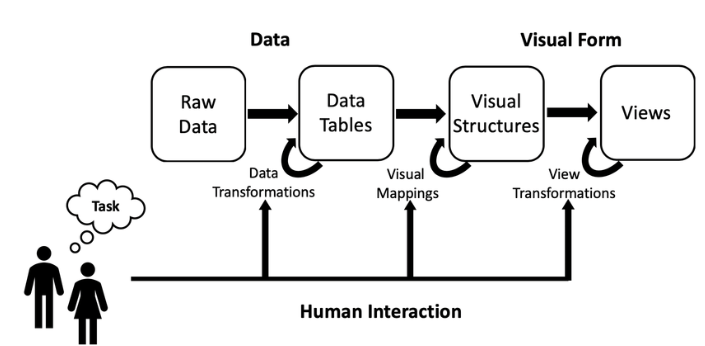
\includegraphics[width=\textwidth]{figure/VizModelDiagram}
\captionof{figure}{Visual Reference model by Card}
\end{center}

While External Cognition describes the advances in graphical technology and how little had been done in the work of the cognitive framework of the discipline, the following citations by Ware attempt to develop the necessary guidelines that are useful for the work done by the perceptual experience.

Colin Ware ``Information Visualization: Perception for Design'' (Ware, 2004) there are four stages of visualization

\begin{itemize}
\tightlist
\item
  The collection and storage of data itself
\item
  The preprocessing design to transform the data into something we can understand
\item
  The display hardware and the graphics algorithms produce the image on the screen.
\item
  The human perceptual and cognitive system
\end{itemize}

The overlapping understanding in the field, while Ware takes the process one step further not just to allow the end user to understand the outcomes but to curate the outcomes with a visual perception of the data that makes the cognitive load easier for the end-user.

A dashboard has much information related to tabular data from multiple sources. Design should be recorded a produced with content that will allow for reproducibility. A dashboard should have some content related to interaction with the user. This interaction can be in multiple forms: toggling through the selection of variables to display uniformly to the use of interaction on the graph and allowing a user to understand best what is being shown in the diagram.

The entire dashboard/Interface should have a human perception piece that is useful for the user to comprehend and use. For example, the dashboard/interface could be more practical if the user is visually overwhelmed.

\begin{itemize}
\tightlist
\item
  Identified the highly relevant from a dashboard design perspective (O'Donnell \& David, 2000)
\end{itemize}

\begin{enumerate}
\def\labelenumi{\arabic{enumi}.}
\tightlist
\item
  Information systems give interaction and feedback
\item
  Type of presentation format to be used
\item
  Differences in the amount of information load.
\end{enumerate}

Information load is essential, as dashboards must provide the right decision cues without overwhelming the user with excess information.

``A decision cue is a feature of something perceived that is used in the interpretation of perception (Choo, 2009),'' where perception is an inferential process as objects in the environment can only be perceived indirectly through available information that has been sensed by the individual (Brunswik, 1952).

Visual complexity and information utility are required. Visual complexity refers to the "degree of difficulty in providing a verbal description of an image.(Heaps \& Handel, 1999), (Olivia, Mack, Shrestha, \& Peeper, 2004)

\begin{itemize}
\tightlist
\item
  Graphs are more suitable for spatial tasks (ex., for comparing a set of values) (Vessey \& Galletta, 1991),(Umanath \& Vessey, 1994); (Vessey, 1994)
\item
  Graphs reduced the negative influence of information overload
\item
  Graphs produced better correlation estimates and decreased time on a task (\textbf{schulzand?} ; Booth \& Siegler, 2006)
\item
  Self-organizing maps and multidimensional scaling did not significantly outperform tabular representations (Huang et al., 2006)
\end{itemize}

The purposes of a dashboard:

\begin{enumerate}
\def\labelenumi{\arabic{enumi}.}
\tightlist
\item
  Consistency
\item
  Monitoring
\item
  Planning
\item
  Communication
\end{enumerate}

``Use interactive visual representations of abstract, non-physically based data to amplify cognition.'' (Card, Mackinlay, \& Shneiderman, 1999)

Visual perception involves two elements - the perceptual and conceptual gist. The perceptual gist refers to the process of the brain when it determines the image properties that provide the structural representation of a scene, like color and texture. The conceptual gist refers to the scene's meaning, which is improved after the perceptual information is received. (Friedman, 1979); (Olivia, Mack, Shrestha, \& Peeper, 2004)

Visual complexity might increase with the quality and range of objects and with varying material and surface styles (Heylighen, 1997).

Repetitive and uniform patterns and existing knowledge of the objects in the scene reduce visual complexity (Olivia, Mack, Shrestha, \& Peeper, 2004).

If the guidelines on our visual information load can be related to statistical terminology, we can consider this the fisher information of visual information load. This load can be used as a metric for balancing the amount of information rather than overloading the consumer.

Visual Data Mining

For data mining to be effective, it is important to include humans in the data exploration process and combine the flexibility, creativity, and general knowledge of the computational power of today's computers. Visual data exploration aims at integrating humans in the data exploration process, applying their perceptual abilities to the large data sets available in today's computer systems.(Keim, 2002)

The visual data exploration process can be seen as a hypothesis generation process:

\begin{itemize}
\tightlist
\item
  The visualizations of the data allow the user to gain insight into the data and come up with new hypotheses
\item
  Along with verification of the hypotheses
\end{itemize}

The main advantages of visual data exploration over automatic data mining techniques from statistics or machine learning are:
- visual data exploration can efficiently deal with highly inhomogeneous and noisy data.
So - visual data exploration is intuitive and requires no understanding of complex mathematical or statistical algorithms or parameters.

Visual Exploration Paradigm, also known as MGV (Massive Graph Visualizer), is an integrated visualization and exploration system for massive multidigraph navigation.(Abello \& Korn, 2002). MGV usually follows a three-step process:

\begin{itemize}
\tightlist
\item
  overview first
\item
  zoom and filter
\item
  details-on-demand
\end{itemize}

The user identifies interesting patterns and focuses on one or more of them. Note that visualization technology does not only provide the base visualization techniques for all three steps but also bridges the gap between the steps.

Visualization Technique Classification:

\begin{itemize}
\tightlist
\item
  Standard 2D/3D displays such as bar charts and x-y plots
\item
  Geometrically transformed displays, such as landscapes and parallel coordinates, as used in a scalable framework
\item
  Icon-based displays such as needle icons and star icons as used in MGV
\item
  Dense pixel displays such as the recursive pattern and circle segments techniques and the graph sketches as used in MGV
\item
  Stacked displays, such as treemaps or dimensional stacking
\end{itemize}

Interaction and distortion techniques allow users to interact directly with the visualizations.

\begin{itemize}
\tightlist
\item
  Projection as used in the Grand Tour System
\item
  Filtering as used in Polaris
\item
  Zooming as used in MGV and scalable framework
\item
  Linking and Brushing as used in Polaris and the scalable framework
\end{itemize}

Design Theory in Information System

The knowledge is distinguished as the fifth of five types of theory:

\begin{enumerate}
\def\labelenumi{\arabic{enumi}.}
\tightlist
\item
  Analyzing \& describing
\item
  Understanding
\item
  Predicting
\item
  Explaining and predicting
\item
  Design and action
\end{enumerate}

A definition of information systems that are suitable for our purposes concerns: "the effective design delivery use and impact of information technology in organizations and society (Avison, Fitzgerald, \& DAWSON, n.d.).

The two paradigms characterize much of the research in the Information systems discipline:

\begin{itemize}
\tightlist
\item
  \emph{Behavioral Science Paradigm} - seeks to develop and verify theories that explain or predict human or organizational behavior (roots in natural science research methods).
\item
  \emph{Data Science Paradigm} - seeks to extend the boundaries of human and organizational capabilities by creating new and innovative artifacts (roots in engineering and the sciences of the artificial).(Simon, 1996)
\end{itemize}

Technology and behavior are not dichotomous in an information system. They are inseparable (Lee, 2000). Information technology (IT) artifacts are broadly defined as:

\begin{itemize}
\tightlist
\item
  constructs (vocabulary \& symbols)
\item
  models (abstractions \& representations)
\item
  methods (algorithms \& practices)
\item
  instantiations (implemented \& prototype systems)
\end{itemize}

These are concrete prescriptions that enable IT researchers and practitioners to understand and address the problems inherent in developing and successfully implementing information systems within organizations ((March \& Smith, 1995); (Nunamaker, Dennis, Valacich, Vogel, \& George, 1991)).

\hypertarget{exploratory-data-analysis}{%
\subsection{Exploratory Data Analysis}\label{exploratory-data-analysis}}

Exploratory Data Analysis (EDA) analyzes and summarizes a dataset to discover patterns, trends, and insights. It is a crucial step in the data analysis process and is often used to identify which variables are essential, what the data looks like, and what the underlying structure of the data is. EDA is typically done using various techniques, such as visualizations, statistical summaries, and data transformations.

On the other hand, Dashboards are interactive interfaces that display data visually to provide insights and support decision-making. Dashboards can be used to monitor key performance indicators, track progress over time, and identify patterns and trends in data. They often display real-time data and can be customized to show the most relevant data to the user.

The connection between EDA and dashboards is that EDA is the process of preparing and understanding the data, which is the first step for building a dashboard, as the data has to be cleaned, transformed, and analyzed to be used efficiently on the dashboard. EDA results can be used to identify the most relevant data and metrics to include in the dashboard and to design the visualizations that will be used to display the data. And also, the EDA process can be used to identify the outliers, patterns, trends, and insights that will be useful to show in the dashboard to support decision-making.

Visualizations of data are essential for exploratory data analysis (EDA) along with model diagnostics.
Plots for EDA are a valuable tool for guiding an analyst in discovering the relationships between variables in their data.
When using plots in model diagnostics, plots help analysts determine whether or not the model is an appropriate way to model.
During the initial EDA stage, an analyst may find that a variable or a covariate is directly related to the dependent variable when looking at a correlation heatmap or a scatterplot.
This will be important to know before starting a linear model analysis.
Much of our general understanding is from introductory statistics courses.
The basic understanding can be formalized to visualize the discovery process.

\hypertarget{eda-through-the-eyes-of-tukey}{%
\subsection{EDA through the eyes of Tukey}\label{eda-through-the-eyes-of-tukey}}

John Tukey was the first to organize the collection and methods associated with philosophy into Exploratory Data Analysis (EDA). John Tukey, creator of stem-and-leaf plot, boxplot-resistant smooth, and the violin plot (also known as rootgram) who taught us to utilize these methods to organize and demonstrate EDA. He was a strong advocate for the importance of EDA as a crucial first step in the data analysis process and emphasized the need for visualization and interactive techniques to understand patterns and relationships in data.

\begin{center}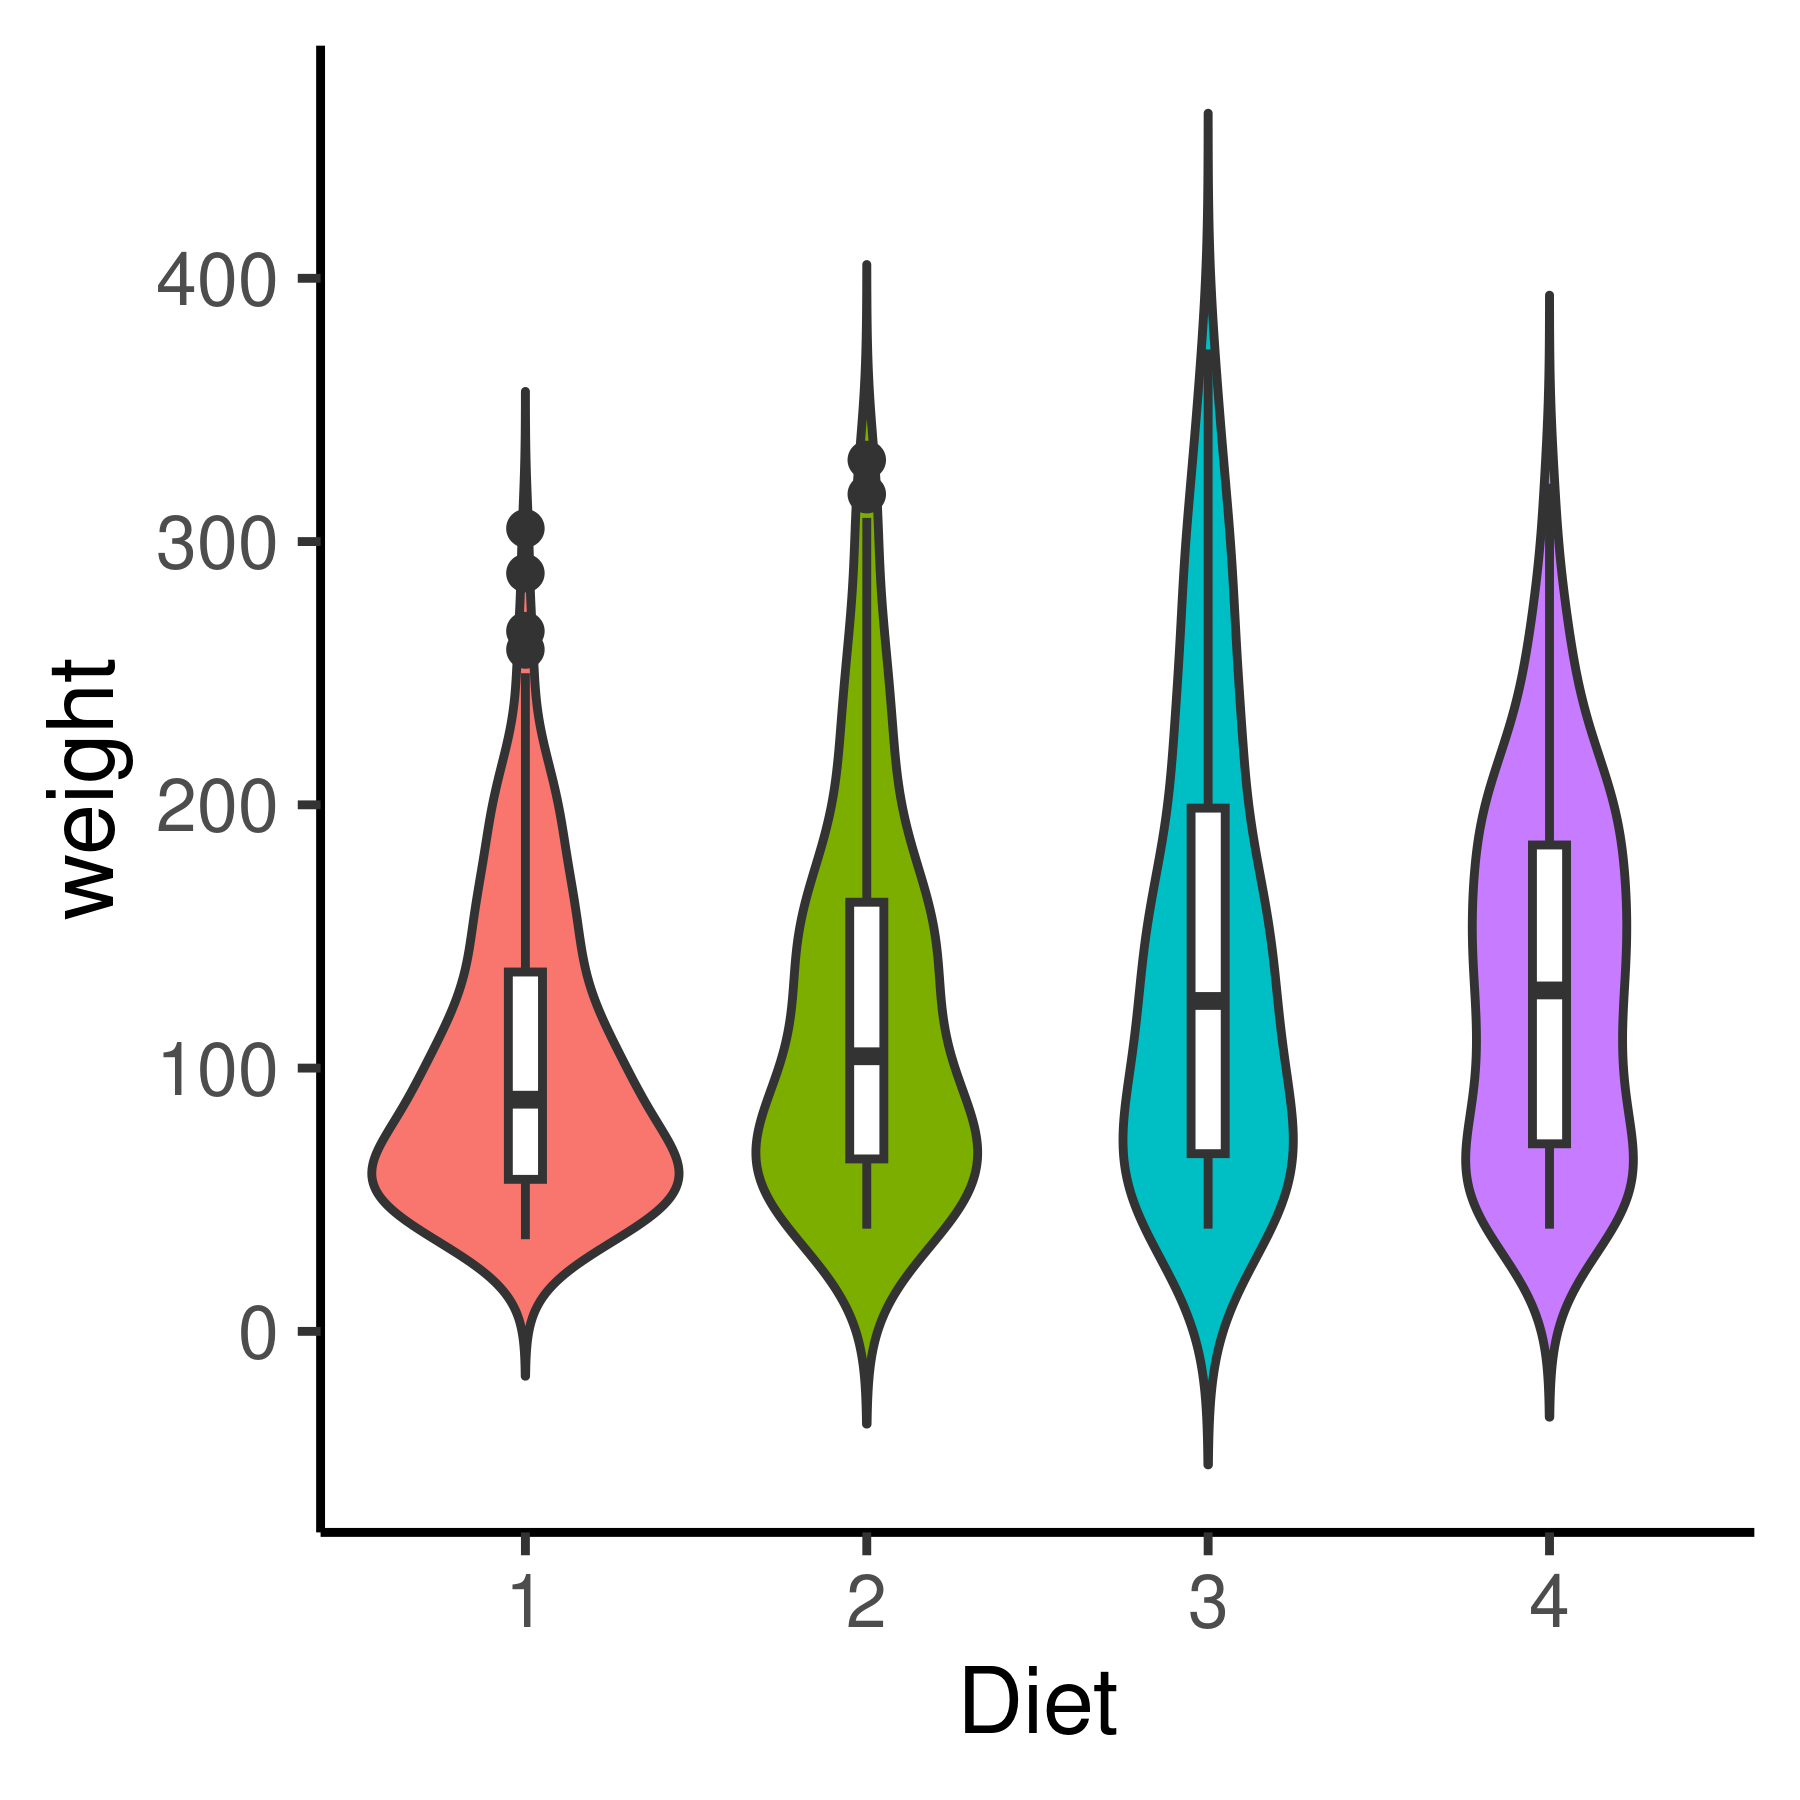
\includegraphics[width=.49\linewidth]{thesis_files/figure-latex/violin_plot-1} 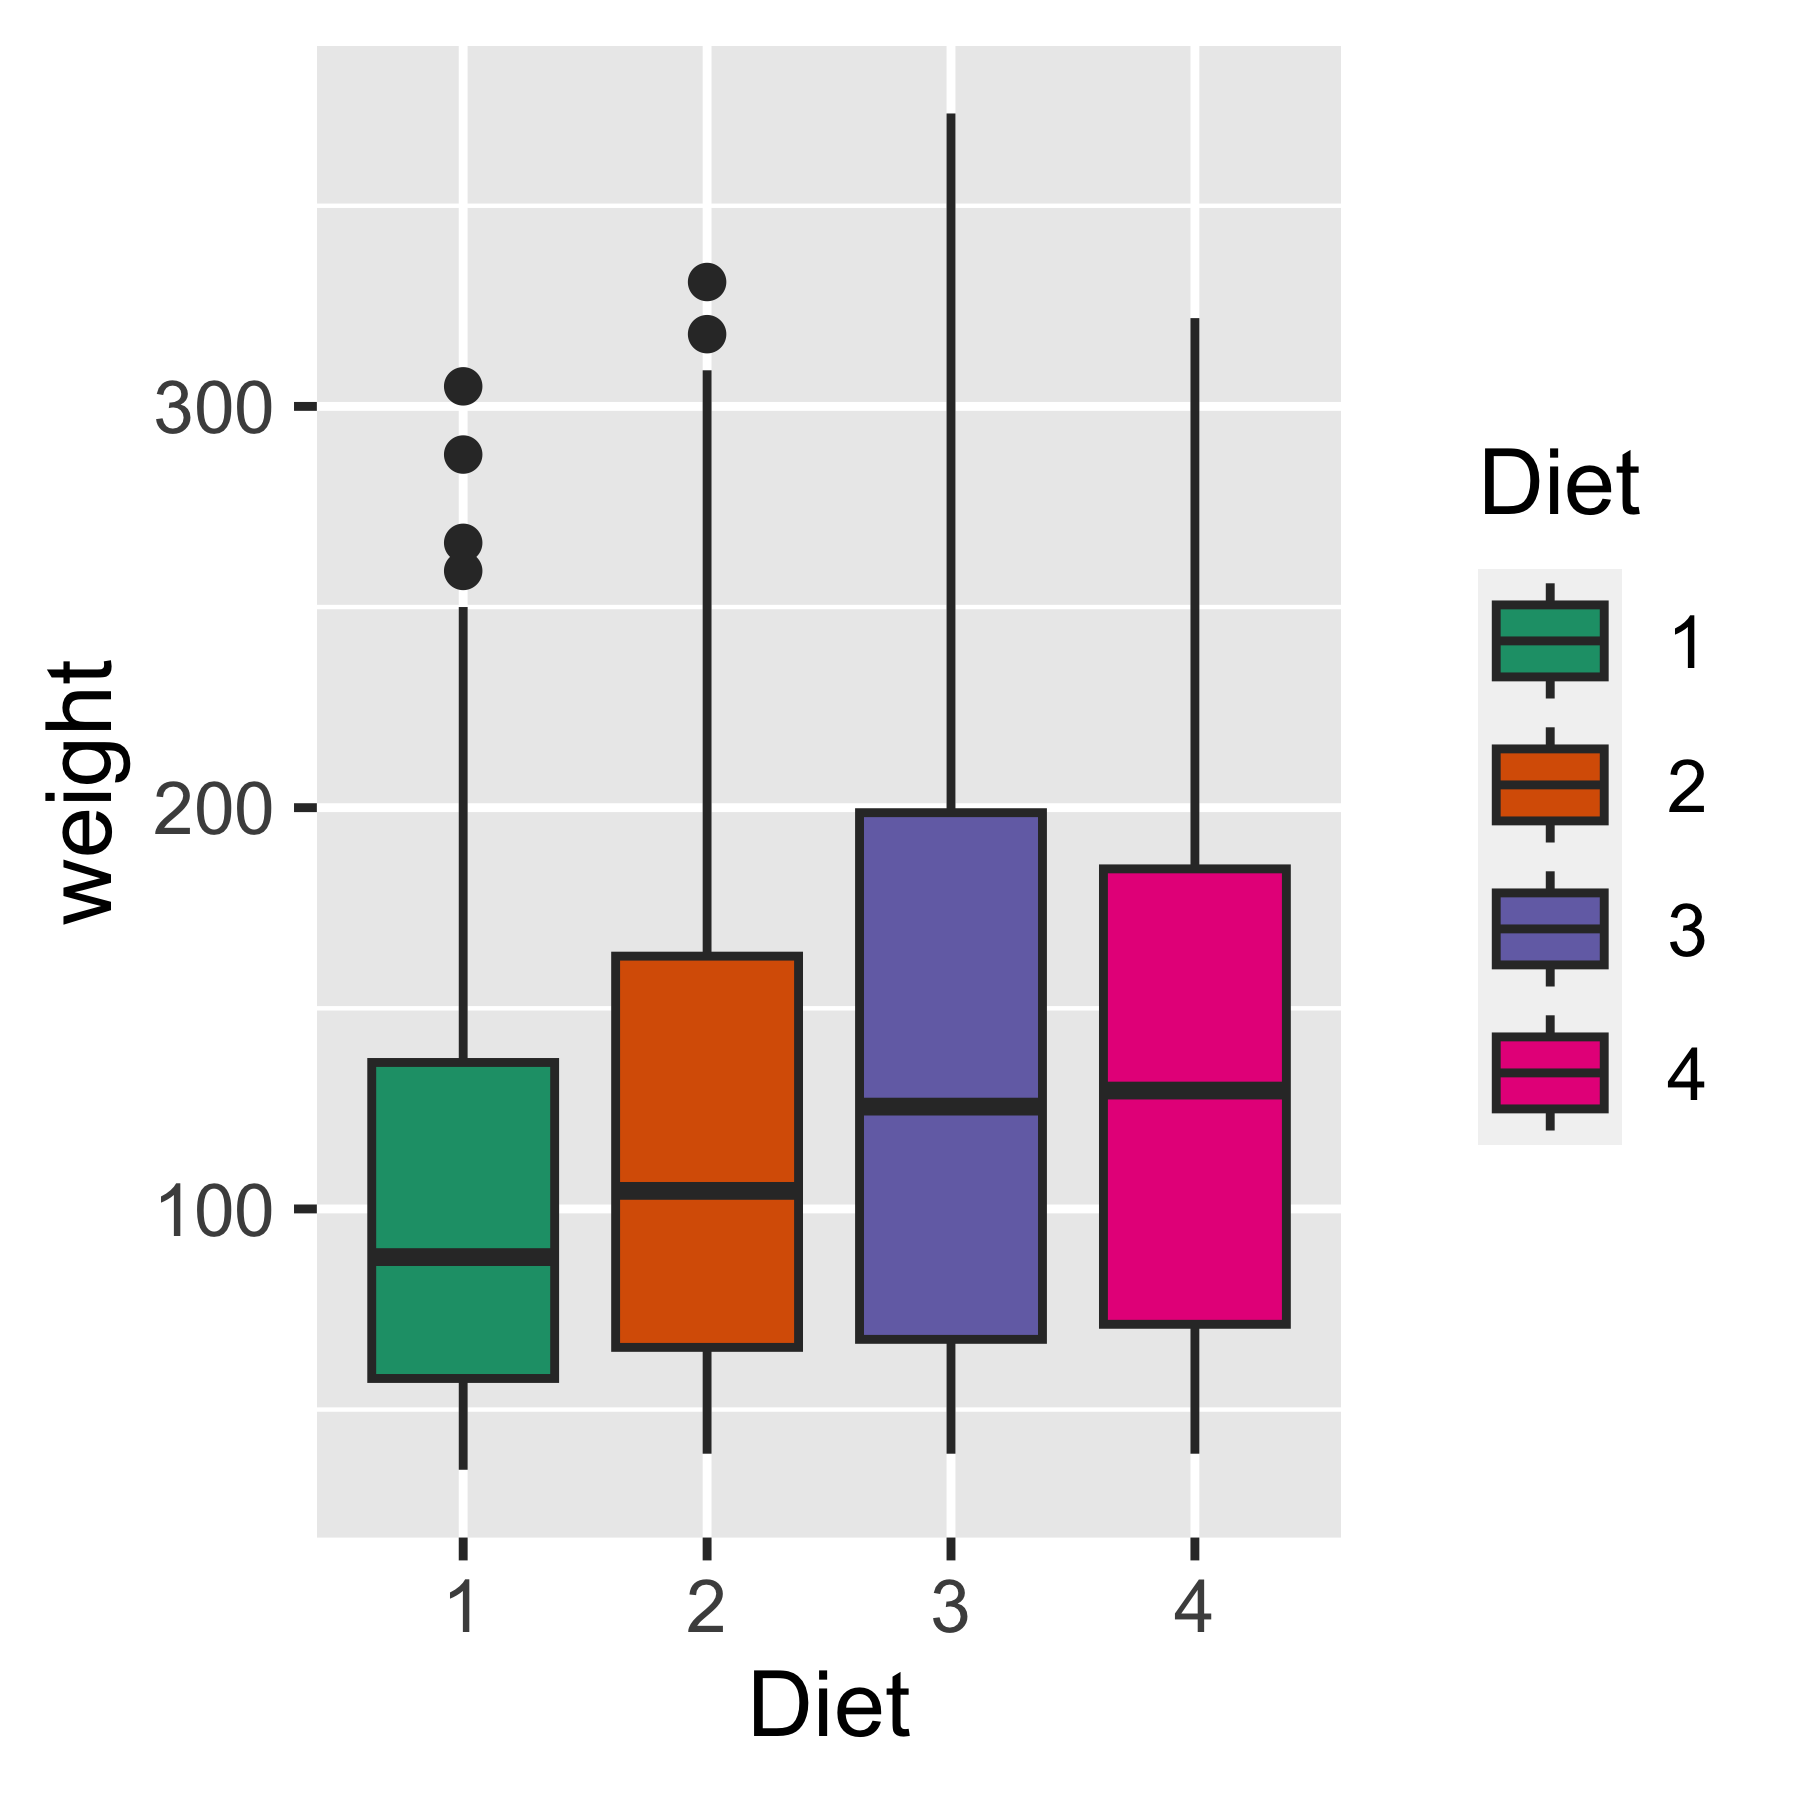
\includegraphics[width=.49\linewidth]{thesis_files/figure-latex/violin_plot-2} \end{center}

Tukey's Principles in EDA:

\begin{enumerate}
\def\labelenumi{\arabic{enumi}.}
\tightlist
\item
  Graphical exploration looking for patterns or displaying fit.
\end{enumerate}

\begin{itemize}
\tightlist
\item
  The method demonstrates things about data that are not understood by a single numeric metric. This has been useful in graphing the data before you develop summary statistics.
\end{itemize}

\begin{enumerate}
\def\labelenumi{\arabic{enumi}.}
\setcounter{enumi}{1}
\tightlist
\item
  Describing the general patterns of the data.
\end{enumerate}

\begin{itemize}
\tightlist
\item
  This step should be insensitive to outliers. In general, think about the types of resistant measures (i.e., median or mean). This step is making sure to determine data patterns.
\end{itemize}

\begin{enumerate}
\def\labelenumi{\arabic{enumi}.}
\setcounter{enumi}{2}
\item
  The natural scale/state that the data are at their best. This will be the step at which the scale of data can be helpful for analysis. The reexpressing data to a new scale by taking the square root or logarithmic scale.
\item
  The mostly known parts of EDA but is done in the way of accessing fit of the data. This is taught in every statistics 101 class. The growth of machine learning and prediction methods have now used residuals more in the toolbox to assessing the best prediction models.
\end{enumerate}

\begin{itemize}
\tightlist
\item
  The idea generally is to determine the deviations in the data from a general pattern by looking at the data from the fit of the data.
\end{itemize}

\begin{verbatim}
## Warning: Groups with fewer than two data points have been dropped.
\end{verbatim}

\begin{verbatim}
## Warning: Removed 1 rows containing missing values (position_stack).
\end{verbatim}

\begin{verbatim}
## `stat_bin()` using `bins = 30`. Pick better value with `binwidth`.
\end{verbatim}

\begin{center}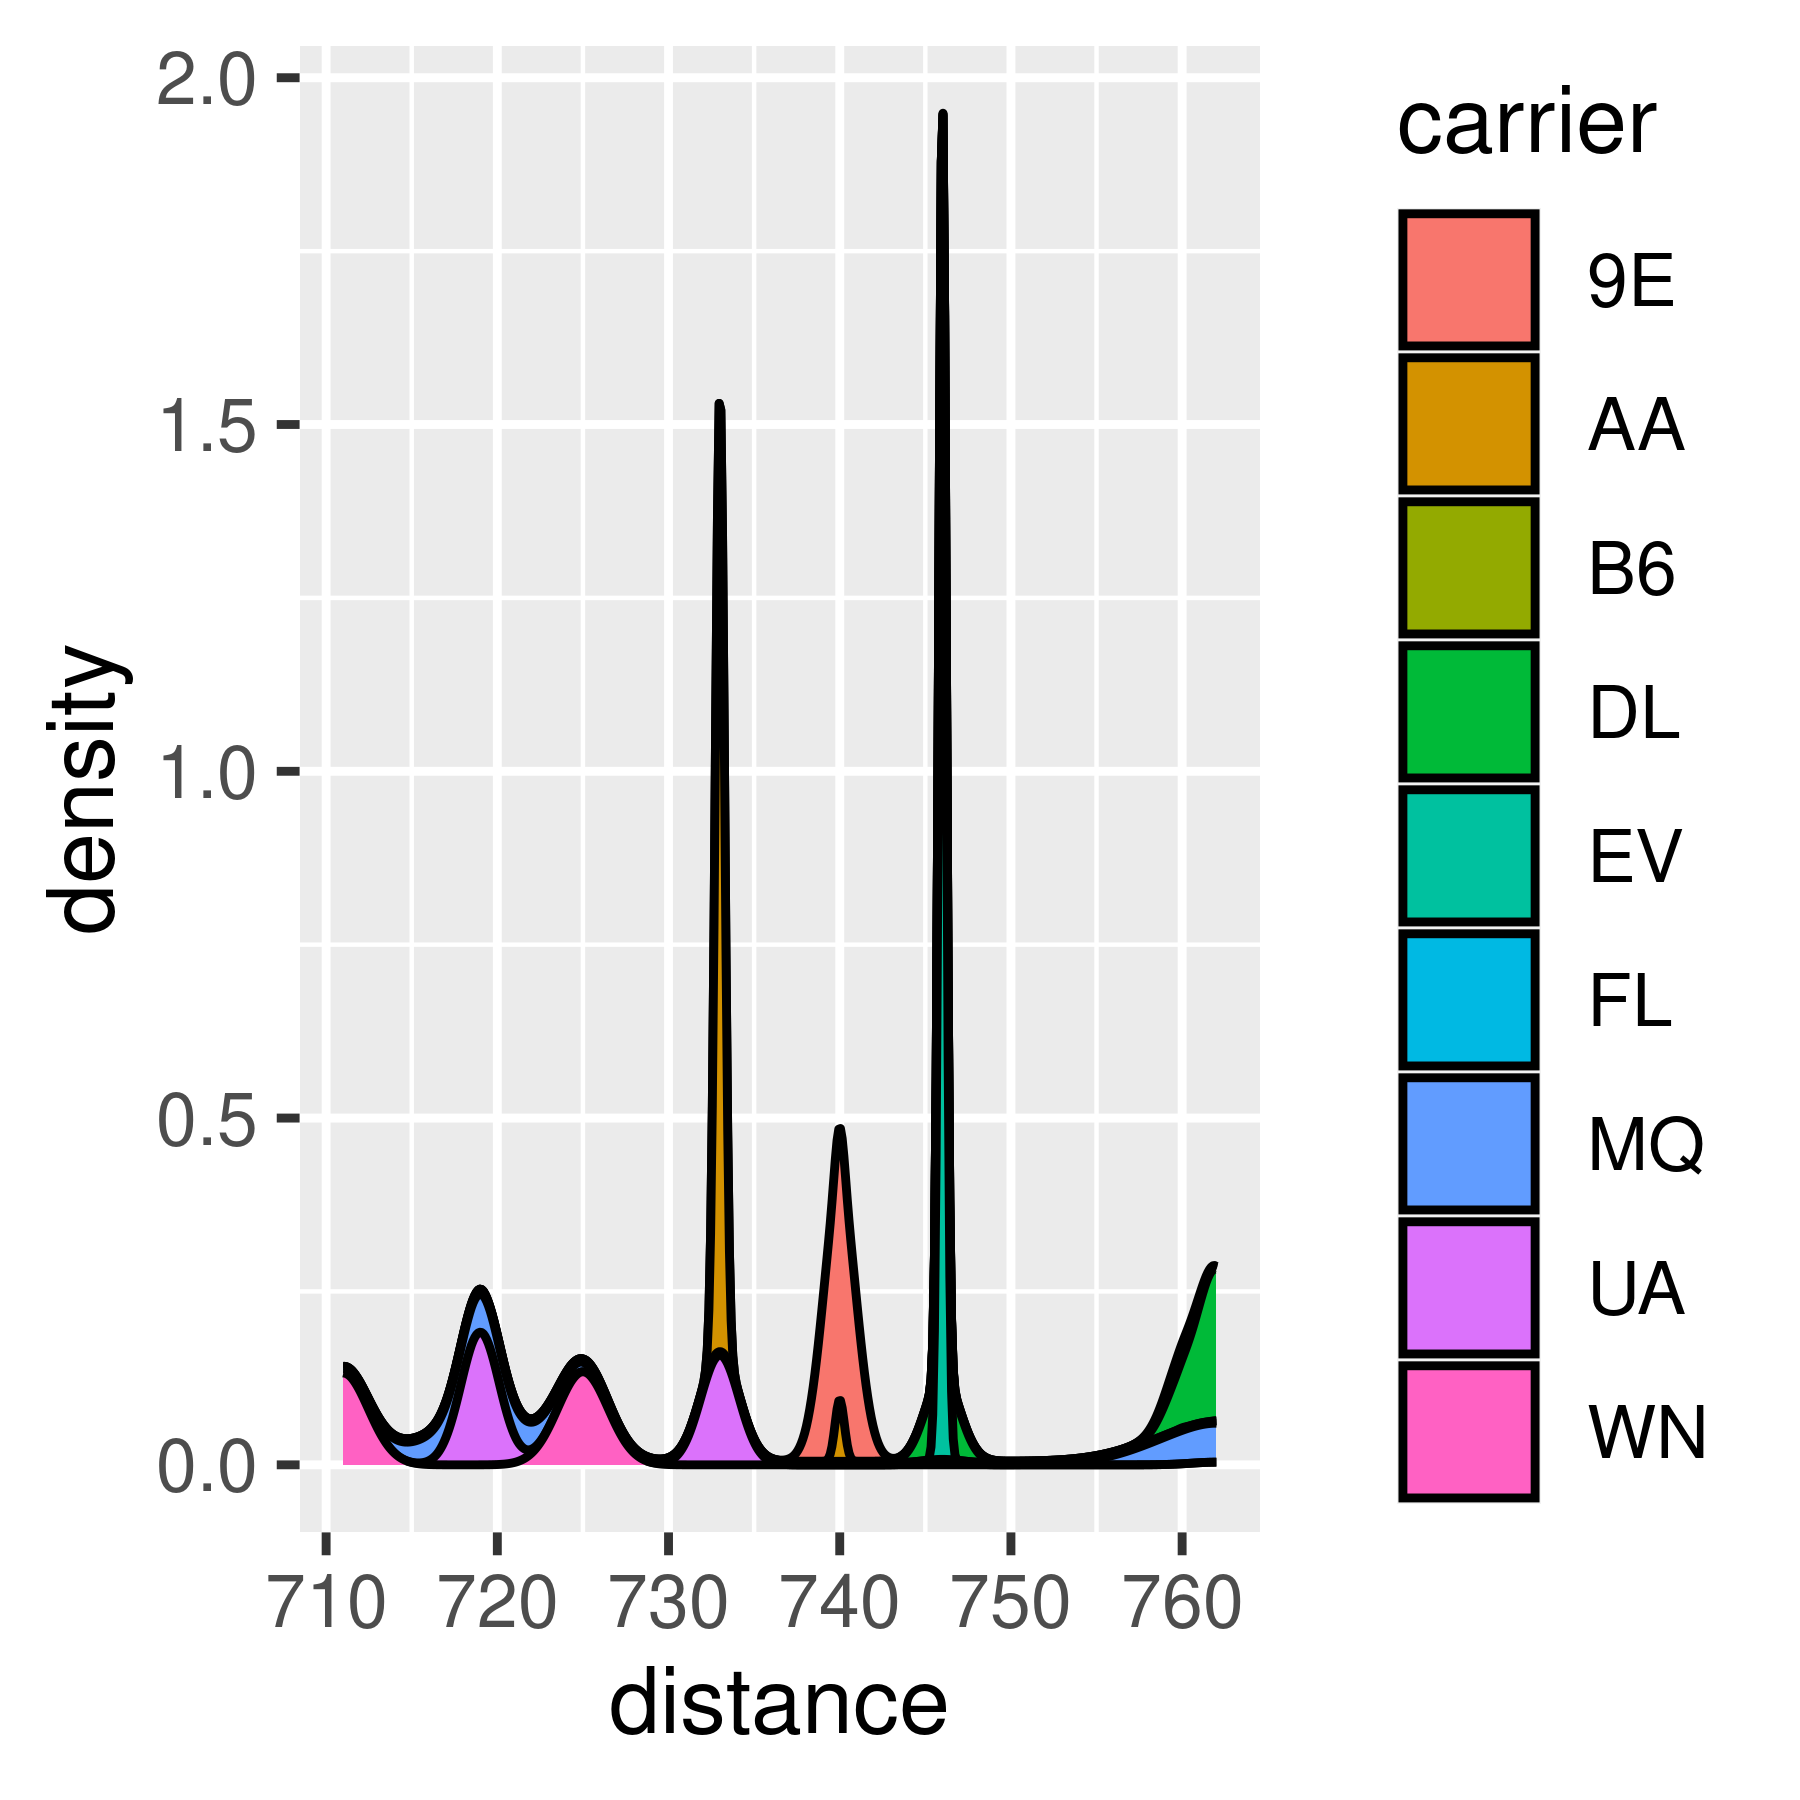
\includegraphics[width=.49\linewidth]{thesis_files/figure-latex/flights_data_example-1} 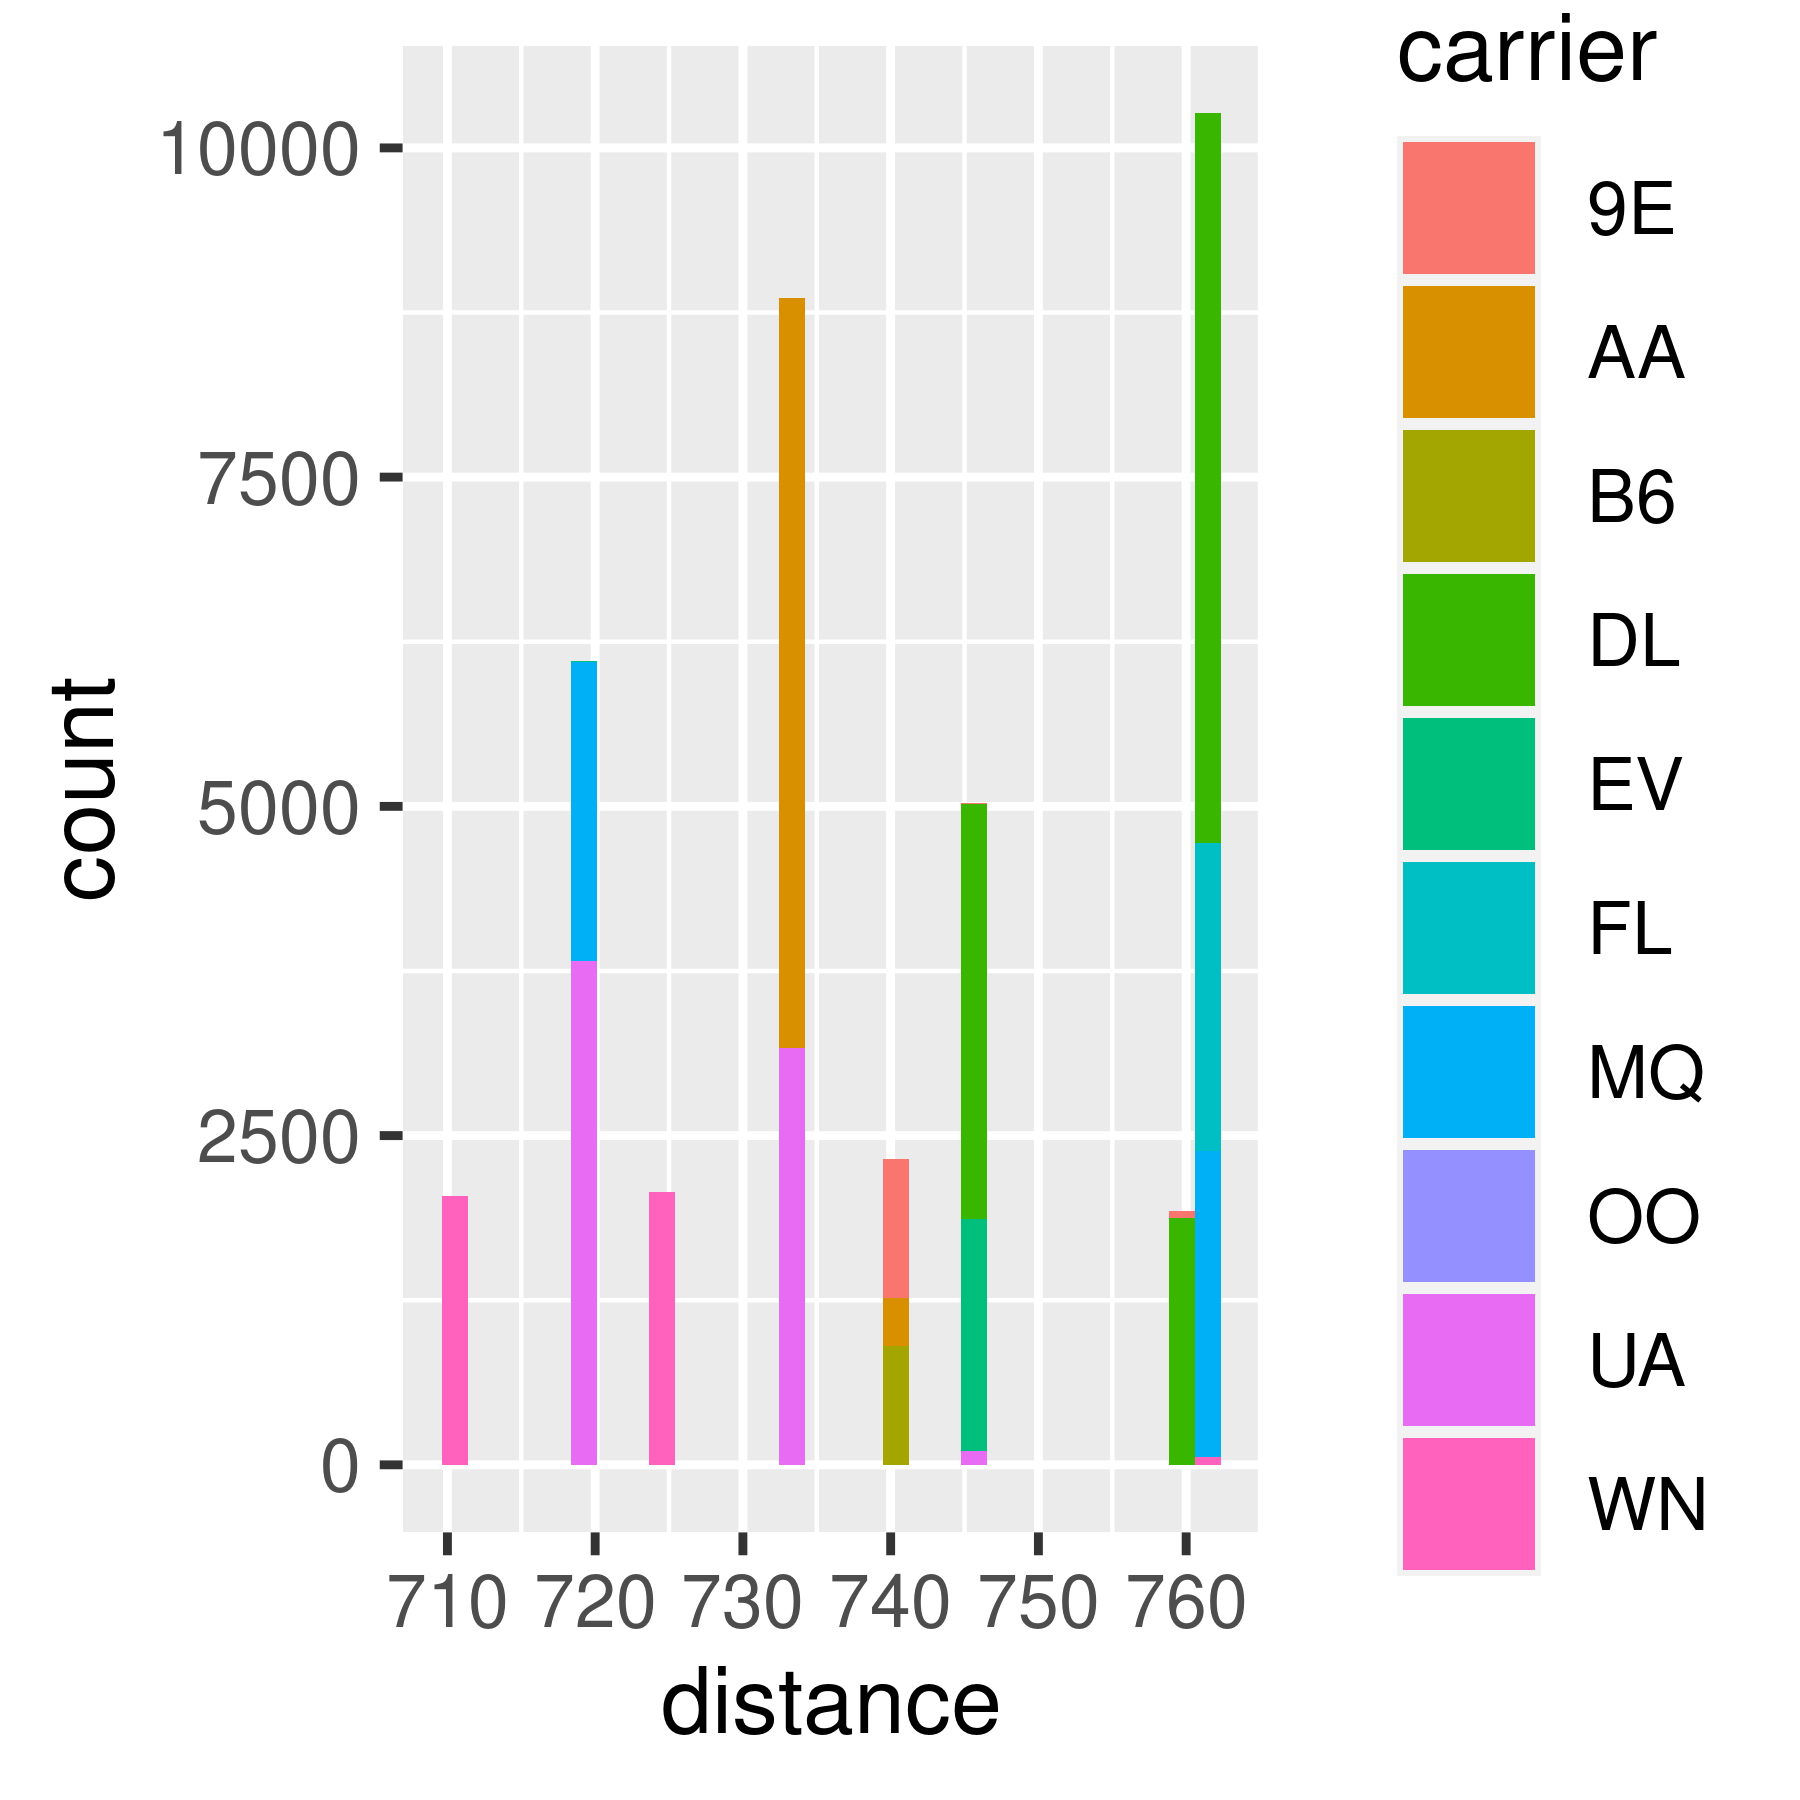
\includegraphics[width=.49\linewidth]{thesis_files/figure-latex/flights_data_example-2} \end{center}

Data Scientists and other analytic professionals often use interactive visualization in the dissemination phase at the end of a workflow, during which findings are communicated to a wider audience. Digital tools are critical to data science and analytics workflows, and current practice spans the following:

\begin{itemize}
\tightlist
\item
  \emph{Data Analysis Tools} - R, Pandas and SAS
\item
  \emph{Data Warehousing Services} - MySQL, MongoDB, or Amazon Redshift
\item
  \emph{Machine Learning Libraries} - scikit-learn o Apache MLlib
\end{itemize}

A typical process typically consists of the following general stages:

\begin{enumerate}
\def\labelenumi{\arabic{enumi}.}
\tightlist
\item
  \emph{Discovery}: Formulating an exciting question and determining the data necessary to answer it.
\item
  \emph{Acquisition}: Locating, organizing, and preparing data to be accessible to the chosen analysis environment.
\item
  \emph{Exploration}: Investigating and analyzing the data set to collect insights and understand the data
\item
  \emph{Modeling}: Building fitting and validating a model that can explain the data set and the observed phenomena
\item
  \emph{Communication}: Disseminating the results to stakeholders in reports, presentations, and charts.
\end{enumerate}

Static Visualization is commonly used in the communication phase of data science workflows, and data scientists sometimes use them as part of the analysis. For example, John Tukey's EDA methods are currently known and well-vetted in the field. However, (Satyanarayan, Moritz, Wongsuphasawat, \& Heer, 2016) began to address this by introducing a high-level grammar of graphics called ``Vega-Lite,'' which presents a set of standardized linguistic rules for producing interactive information visualizations using a concise JSON format for data to be represented by the grammar. Vega-Lite has been directly implemented in R via the \texttt{ggvis} package using the same - albeit slightly lower-level.

\hypertarget{grammar-of-graphics}{%
\subsection{Grammar of Graphics}\label{grammar-of-graphics}}

The grammar of graphics (gg of ggplot2) is a theory that is well-defined for creating statistical graphics with work from Wilkinson (\textbf{Wilkinson1999?}) and Hadley Wickham (Wickham, 2016). The Grammar of Graphics is a framework for understanding the structure of statistical graphics developed by Leland Wilkinson. It proposes that any statistical graphic can be broken down into a set of essential components, or ``grammar,'' that can be combined in different ways to create a wide range of visualizations.

Grammar of graphics is defined as the framework which follows a layered approach to describe and construct visualizations or graphics in a structured manner.

The components of the grammar of graphics include:

\begin{itemize}
\tightlist
\item
  Data: The raw data being visualized represents a set of observations or values.
\item
  Aesthetic Mappings: The mapping of data variables to visual properties such as position, color, shape, and size.
\item
  Scales: The mapping of data values to visual values, such as mapping a numerical value to a bar height.
\item
  Geometries: The basic shapes representing the data, such as points, lines, bars, and histograms.
\item
  Facets: The plot division into multiple subplots, each representing a different subset of the data.
\end{itemize}

For example, a bar chart can be created by mapping a categorical variable to the x-axis, mapping a numerical variable to bar heights, and using rectangular bars as the geometry. For example, mapping two numerical variables can create a scatter plot to the x and y positions and use points as the geometry. Finally, the Grammar of Graphics provides a systematic way of thinking about visualizations, making it easier to choose the appropriate visual representation for a given dataset.

\begin{center}
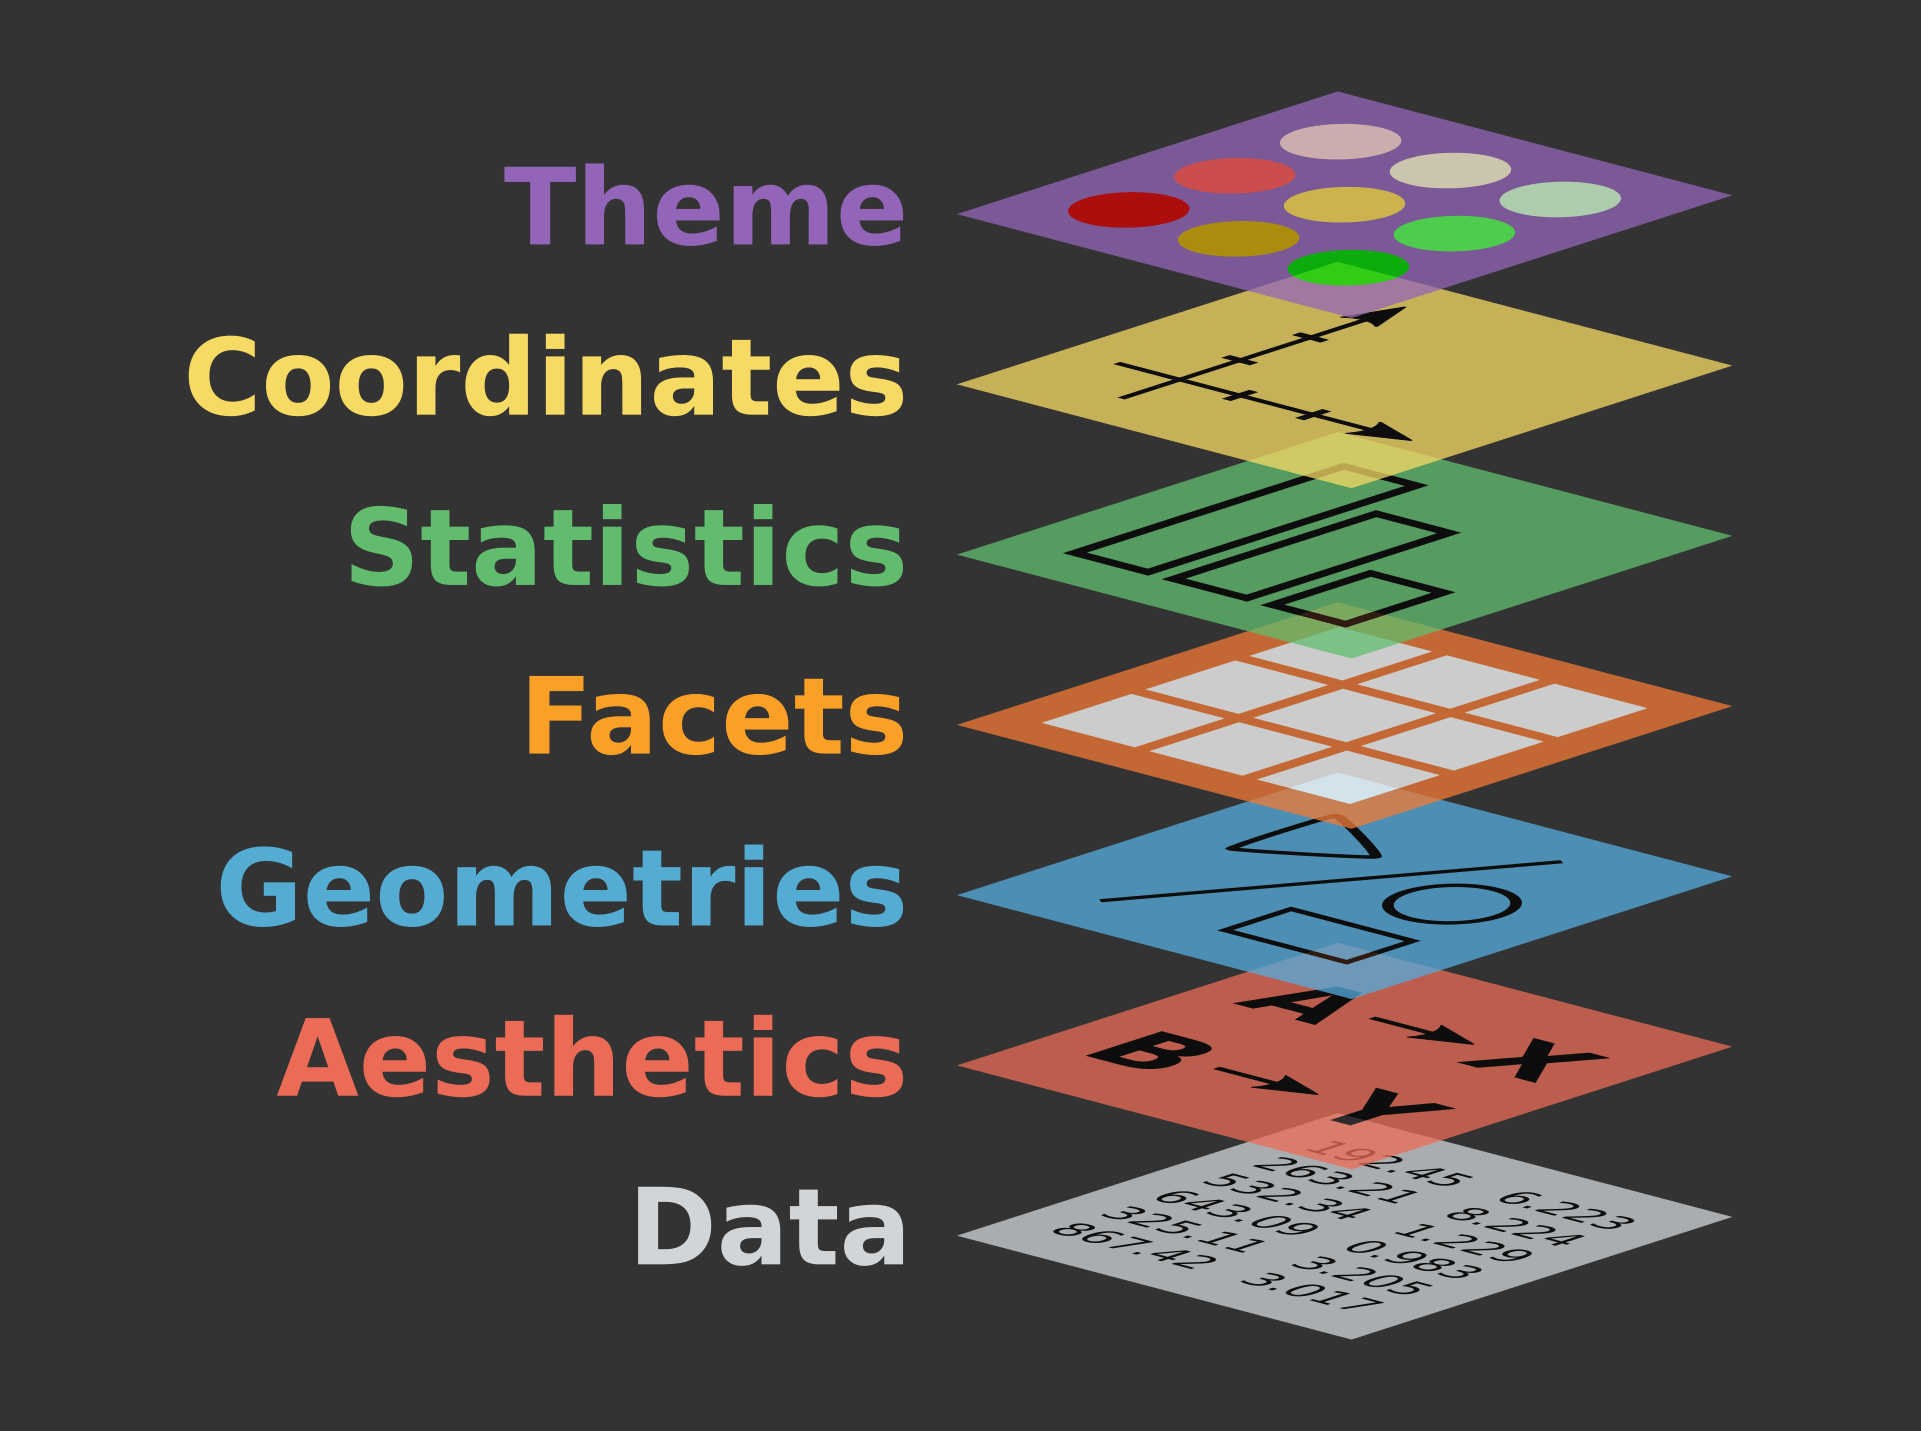
\includegraphics[width=\textwidth]{figure/gglayers}
\captionof{figure}{Grammar of Graphics Diagram of Wickham and Wilkinson's work}
\end{center}

\begin{center}\rule{0.5\linewidth}{0.5pt}\end{center}

\begin{center}
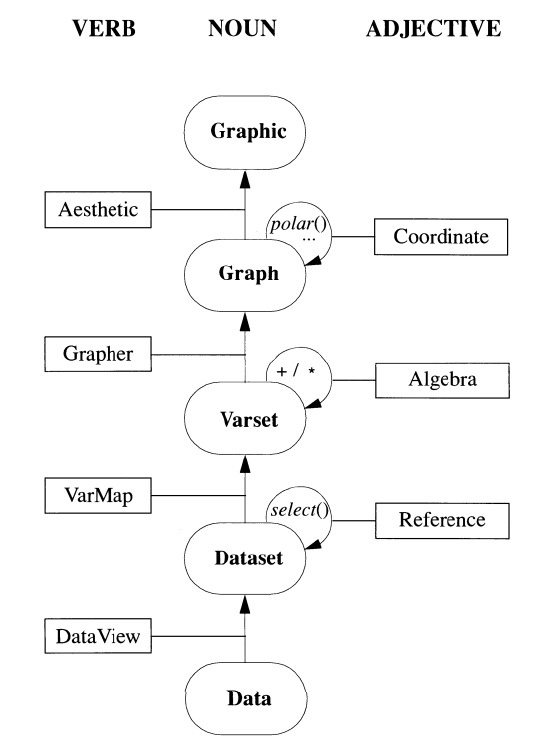
\includegraphics[width=\textwidth]{figure/graphic-flowchart}
\captionof{figure}{Grammar of Graphics Diagram of Wickham and Wilkinson's work}
\end{center}

\hypertarget{big-data-and-graphical-solutions}{%
\subsection{Big Data and graphical solutions}\label{big-data-and-graphical-solutions}}

Big Data Analytics examines large and complex data sets, or ``big data,'' to uncover hidden patterns, correlations, and other insights. Big data analytics aims to help organizations make informed decisions by transforming large and complex data into actionable information. The use of big data analytics can provide organizations with a competitive advantage by enabling them to quickly and accurately analyze large volumes of data, identify trends and patterns, and make informed decisions. This can help organizations to improve their operations, identify new opportunities, and make more accurate predictions about future events.

Graphical solutions for big data refer to visual representations to help analyze and understand large and complex data sets. The following are some standard graphic solutions for big data:

\begin{itemize}
\tightlist
\item
  Interactive dashboards: Dashboards provide a visual overview of critical metrics and KPIs, allowing users to interact with the data in real time. Dashboards can display large amounts of data clearly and concisely, making it easier to identify trends and patterns.
\item
  Scatter plots: Scatter plots visualize the relationship between two or more variables and can identify correlations, outliers, and clusters in big data sets.
\item
  Heatmaps: Heatmaps are used to visualize data distribution across two dimensions. They can be used to identify areas of high and low density in big data sets, making it easier to spot trends and patterns.
\item
  Treemaps: Treemaps are used to visualize hierarchical data structures. They can be used to visualize large data sets in a compact and organized manner, making it easier to identify relationships between different data points.
\item
  Network graphs: Network graphs are used to visualize relationships between data points. They can be used to identify connections and relationships in big data sets, making it easier to spot patterns and trends.
\end{itemize}

Using graphical solutions for big data is to help organizations quickly and easily understand large amounts of data, identify patterns and relationships, and make informed decisions. These visual representations can provide a more immersive and engaging experience, making it easier to uncover insights that might not be immediately apparent from raw data.

Many companies and organizations use big data and graphical solutions to make data-driven decisions, identify new opportunities, and gain a competitive advantage. New technologies like data visualization software, cloud computing, and machine learning make analyzing and presenting big data more accessible and efficient.

\hypertarget{eda-through-the-eyes-of-big-data-and-big-data-analytics}{%
\subsubsection{EDA through the eyes of Big Data and Big Data Analytics}\label{eda-through-the-eyes-of-big-data-and-big-data-analytics}}

Big Data Analytics is where advanced analytic techniques are applied to big data sets. Big Data Analytics based on extensive data samples reveals and leverage business change. The larger the data set, the more difficult it becomes to manage. This paradigm has only become more of the pieces of data exploration since tabular data is growing.

\hypertarget{interactive-graphics}{%
\subsection{Interactive Graphics}\label{interactive-graphics}}

The area of interactive graphics is still very much a work in progress despite existing as a field of research since the late 1960s---developments are driven partly by new technology, such as \texttt{d3} (Bostock, Ogievetsky, \& Heer, 2011). Visualizations are more than just a picture. They are now a tool that facilitates analytic activity through different modes of interaction. (Yi, Kang, Stasko, \& Jacko, 2007). Visualization is context-free, as it can mean different things to different people depending on the situation (Parsons \& Sedig, 2014).

The van Wijk Simple Visualization Model is a diagrammatic representation that provides a simple and effective way to understand and visualize the flow of information and data through a system. It is a commonly used tool in Exploratory Data Analysis (EDA), which is the initial step in the data analysis process. The van Wijk model can be used to represent the flow of data from data sources, through intermediate processing stages, to the final visualization of results. van Wiij's (Van Wijk, 2005) simple visualization model shows how insights are generated as the human participates in a feedback loop between reading and interacting with visualization.

This model is also context-free, allowing for the focus to be on the feedback loops between visualization and the user.

\begin{center}
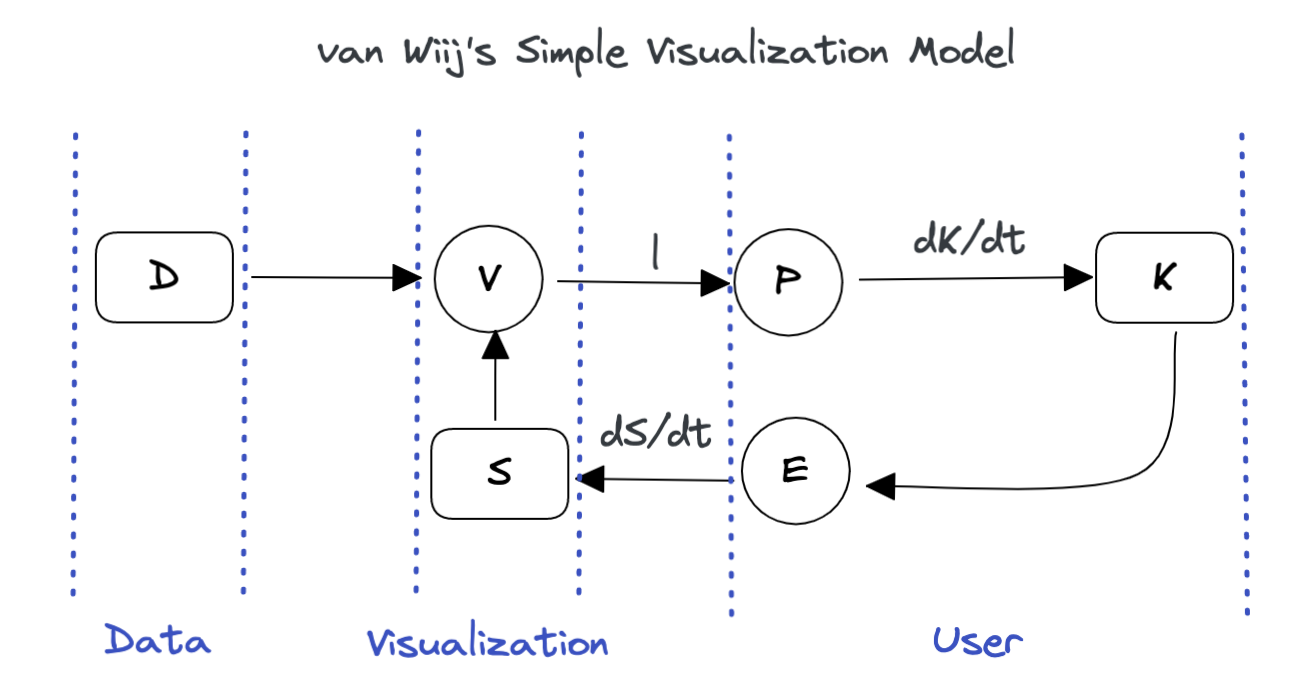
\includegraphics[width=\textwidth]{figure/vanWiijSimpleModel}
\captionof{figure}{van Wiij Simple Visualization Model}
\end{center}

Interaction allows the user to define what data they see and how they see it, creating a dialogue between the user and the system. Theories behind visual representation include:

\begin{itemize}
\tightlist
\item
  graphical comprehension ((Cleveland \& McGill, 1984))
\item
  preattentive processing ((Ware, 2012))
\item
  gestalt theory ((Few, 2009))
\item
  graphical excellence ((\textbf{tufte2001?}))
\end{itemize}

Theories behind the manipulation of visualizations include but are not limited to:

\begin{itemize}
\tightlist
\item
  cognitive fit ((Vessey \& Galletta, 1991))
\item
  visual perceptual approaches ((\textbf{baker2009?}))
\item
  human information processing
\end{itemize}

As interactive visualizations play a more significant role in information systems, designers must know what tasks, visual representations, and interaction techniques are available and how they work to facilitate analytical reasoning. They must decide on the most effective visual representation without being able to estimate every user's ability to read and interpret the visualization

Interactive visualization is a commonly used tool in Exploratory Data Analysis (EDA), which is the initial step in the data analysis process. The goal of EDA is to gain a high-level understanding of the data and to identify patterns, relationships, and anomalies in the data.

Visualizations have become more effective in recent years due to the pandemic and the Johns Hopkins University COVID-19 Dashboard (Dong E, 2022) \href{https://coronavirus.jhu.edu/map.html}{Dashboard}.
We were glued to our computers, TVs, and phones for most of the world.
As a result, we watched the dashboard change in real-time to adapt to the users' needs.
In part to data growth and changing, the dashboard, as well as the visualizations, were needed in a condensed platform.
The need to be concise and vastly informative is a struggle regarding data visualizations.

The human brain can only take in a set amount of data from a table or a paragraph. \svp{references?}
The space of infographics has been a much better way of looking at data on a creative scale.(Wickham, 2013)
While this may be a way of seeing the data in a friendly way, infographics need to include an interactive piece of data that many people would like to explore.

The relationship between the van Wijk Simple Visualization Model and Human-Computer Interaction (HCI) lies in the area of data visualization. The van Wijk Model provides a framework for understanding how information and data flow through a system to be displayed to the user. In the context of HCI, the model helps to understand how data is processed, transformed and presented to the user in a way that is intuitive, informative and engaging. The model helps to identify the various steps involved in the visualization process, from the collection and processing of data to the presentation of results. By doing so, it supports the design of more effective and user-friendly visualizations, which can enhance the overall user experience.

\hypertarget{human-computer-interaction-hci-uxui-design}{%
\section{Human Computer Interaction (HCI) \& UX/UI Design}\label{human-computer-interaction-hci-uxui-design}}

\hypertarget{user-analysis}{%
\subsection{User analysis}\label{user-analysis}}

User analysis is a crucial step in the design of user interfaces, especially in Human-Computer Interaction (HCI) and User Experience (UX) design. It involves studying the users of a system to understand their needs, goals, and behaviors. The purpose of user analysis is to create interfaces that are easy to use, efficient, and effective for the intended audience.

Several methods can be used to conduct user analysis:

\begin{itemize}
\tightlist
\item
  Interviews: This involves conducting in-depth interviews with users to understand their needs, goals, and workflows.
\item
  Surveys involve sending out surveys to users to gather data on their needs and preferences.
\item
  Observations: This involves observing users as they complete tasks with the interface to understand their behaviors and workflows.
\item
  Personas: This is a method of creating fictional characters that represent the different types of users; it helps to understand the users' needs and goals.
\item
  Scenarios: This is a method of creating stories that describe how a user might interact with a system; it helps to understand the context and the user's needs.
\item
  Focus groups: This is a method of gathering a small group of users and facilitating a discussion to understand the users' needs and goals.
\item
  Contextual inquiry: This is a method of visiting the users in their work environment and observing them while they work; it helps to understand the context and the user's needs.
\end{itemize}

The results of user analysis can be used to inform the design of the interface, including the layout, navigation, and functionality. It can also be used to identify areas of the interface that are confusing or difficult to use and to make recommendations for improvements. User analysis is an iterative process, and it should be done in multiple stages of the design process to ensure that the final product is tailored to the users' needs.

\hypertarget{protocols-for-testing-design}{%
\subsection{Protocols for testing design}\label{protocols-for-testing-design}}

Several protocols and methods can be used to test the design of a dashboard or other visual display. Some of these include:

\begin{itemize}
\tightlist
\item
  Usability testing: This involves having users interact with the dashboard and providing feedback on its usability, including how easy it is to navigate, understand, and use.
\item
  Cognitive walkthrough: This involves having experts in human-computer interaction evaluate the dashboard, focusing on the cognitive processes required to use it effectively.
\item
  Eye-tracking: This involves using technology to track the users' gaze and interactions, to understand the user's focus and attention on the dashboard elements.
\item
  A/B testing: This involves creating two versions of the dashboard, each with slightly different design elements, and comparing the results to see which design is more effective.
\item
  Surveys: This involves asking users to complete a survey that measures their satisfaction and understanding of the dashboard and to provide feedback on improvements.
\item
  Heat maps: This involves using heat maps to track where users are clicking on the dashboard to identify which elements are being used the most and which are being ignored.
\item
  Card sorting: This is a method to understand the users' mental models and how they would like to organize and categorize the data; it is helpful to understand how to structure the dashboard navigation.
\end{itemize}

These are just a few examples of the many protocols and methods that can be used to test the design of a dashboard. The selection of the appropriate way will depend on the specific goals of the testing and the resources available.

Remember that the user's feedback is crucial in the testing process; it will provide the necessary insight to improve the design and make it more efficient.

\hypertarget{general-dashboard-stuff}{%
\section{General Dashboard stuff}\label{general-dashboard-stuff}}

Dashboards can help understand and support many data types in essential business objectives. There are many different ways to label and utilize dashboards in different kinds.

Dashboards are cognitive tools that should be used to improve understanding of data, which should help people visually find relationships, trends, patterns, and outliers. Most importantly, dashboards should leverage people's visual cognitive capabilities.

EDA refers to methods and procedures for exploring the data space to learn about a data set. By analogy, exploratory modeling analysis (EMA) refers to methods and procedures for exploring the space of models which may be fit to a data set.

Interactive graphics are excellent for EDA; they are designed for exploring rather than presenting information (and more) and can be obtained by directly querying the graphic (Unwin, Volinsky, \& Winkler, 2003).

\begin{itemize}
\tightlist
\item
  PCPs enable the display of multi-dimensional data in two-dimensional space.
\item
  There must be some loss of information, but this can be partly counteracted by varying the order of the axes.
\item
  Interactivity is valuable for reordering the axes flexibly and fast.
\item
  Interaction is valuable for dealing with the dense mass of lines produced by large data sets.
\end{itemize}

Being able to select subgroups of cases, highlight the chosen lines, and switch between different subgroups all assist in interpreting the otherwise intricate displays which arise.

Cowan (Cowan, 2001) suggested that the average person can only hold two to six pieces of information in their attention. People can develop detailed understandings of reality, which is infinitely complex.

Cognitive structures consist of mental models and their relationships ((Rumelhart \& Ortony, 1976), (Carley \& Palmquist, 1992), (\textbf{jonassen1996?})). Mental models have been studied under several different names, which are displayed in the following image of Cognitive Structures:

\begin{itemize}
\tightlist
\item
  Frames: (\textbf{Goffman1974?}); (\textbf{Minsky1975?}); (\textbf{Rudolph2003?}); (\textbf{Smith1986?}); (\textbf{Klein2003?})
\item
  Scripts: (\textbf{ShankandAbelson1977?})
\item
  Protoypes: (\textbf{RoschandMervis1975?});(\textbf{Rosch1977?}); (\textbf{Smith1978?})
\item
  Schemas: (\textbf{Bartlett1932?}); (\textbf{Neisser1976?}); (\textbf{Piagetandcook1952?})
\end{itemize}

A schema is a mental model containing a breadth of information about a specific object or concept. Schemas are organized into semantic networks based on their relationships to other schemas (Wertheimer, 1938), (Rumelhart \& Ortony, 1976). This arrangement helps the brain process its experiences instead of storing every sensory observation; the brain only needs to maintain its schemas, which are good summaries of all previous observations. Some ``memories'' may even be complete recreations built with a schema (Bartlett \& Remembering, 1932), (Klein, Phillips, Rall, \& Peluso, 2007)

(Wixon, Holtzblatt, \& Knox, 1990) introduce ``contextual design'' as a systems development method in which the researcher partners with the user at the user's place of work to ``develop a shared understanding'' of the user's activities, and they define contextual inquiry as the first part of the broader process. Contextual inquiry is the data collection step of the field research element of the contextual design method, and it emphasizes four essential principles:

\begin{enumerate}
\def\labelenumi{\arabic{enumi}.}
\tightlist
\item
  The context of the activity being performed by the user
\item
  The partnership between the researcher and the participant
\item
  The spoken verification that the investigator's interpretation of the activity matches the user's
\item
  The focus of the study is central to the approach taken by the interviewer
\end{enumerate}

(Kandel, Paepcke, Hellerstein, \& Heer, 2012) conducted what might be considered a contextual interview study similar to ours in that they analyzed data scientists' self-reported work processes. Kandal proposes three main archetypes that data scientists may be classed into the following:

\begin{itemize}
\tightlist
\item
  Hackers: who build processes chaining together multiple programming languages of different types (analytical, scripting, and database languages) and use visualization in various environments.
\item
  Scripters: who perform most of their analysis in an analytical environment (e.g., R or Python) and execute the most complex statistical modeling of the types but who do not performstatements their ETL
\item
  Application Users: who performed most or all of their work in an application such as Excel or SPSS and, like scripters, relied on others (namely, their organizations' IT departments) for ETL.
\end{itemize}

\hypertarget{conclusion}{%
\subsection{Conclusion}\label{conclusion}}

\hypertarget{rmd-basics}{%
\chapter{Chapter Paper on Rural Shrink Smart Manuscript submitted to Journal of Data Science Special Issue}\label{rmd-basics}}

Placeholder

\hypertarget{abstract}{%
\section{Abstract}\label{abstract}}

\hypertarget{introduction-1}{%
\section{Introduction}\label{introduction-1}}

\hypertarget{data-description}{%
\section{Data Description}\label{data-description}}

\hypertarget{dashboard-design-considerations}{%
\section{Dashboard Design Considerations}\label{dashboard-design-considerations}}

\hypertarget{guiding-design-principles}{%
\section{Guiding Design Principles}\label{guiding-design-principles}}

\hypertarget{dashboard-design-process}{%
\section{Dashboard Design Process}\label{dashboard-design-process}}

\hypertarget{dashboard-components}{%
\subsection{Dashboard Components}\label{dashboard-components}}

\hypertarget{initial-draft}{%
\subsection{Initial Draft}\label{initial-draft}}

\hypertarget{redesign}{%
\subsection{Redesign}\label{redesign}}

\hypertarget{discussion}{%
\section{Discussion}\label{discussion}}

\hypertarget{future-work}{%
\section{Future Work}\label{future-work}}

\hypertarget{conclusions}{%
\section{Conclusions}\label{conclusions}}

\hypertarget{math-sci}{%
\chapter{Chapter 2 Stuff}\label{math-sci}}

Placeholder

\hypertarget{introduction-2}{%
\section{Introduction}\label{introduction-2}}

\hypertarget{dashboard-design-considerations-1}{%
\section{Dashboard Design Considerations}\label{dashboard-design-considerations-1}}

\hypertarget{guiding-design-principles-1}{%
\subsection{Guiding Design Principles}\label{guiding-design-principles-1}}

\hypertarget{ref-labels}{%
\chapter{Tables, Graphics, References, and Labels}\label{ref-labels}}

Placeholder

\hypertarget{tables}{%
\section{Tables}\label{tables}}

\hypertarget{figures}{%
\section{Figures}\label{figures}}

\hypertarget{footnotes-and-endnotes}{%
\section{Footnotes and Endnotes}\label{footnotes-and-endnotes}}

\hypertarget{cross-referencing-chapters-and-sections}{%
\section{Cross-referencing chapters and sections}\label{cross-referencing-chapters-and-sections}}

\hypertarget{bibliographies}{%
\section{Bibliographies}\label{bibliographies}}

\hypertarget{anything-else}{%
\section{Anything else?}\label{anything-else}}

\hypertarget{conclusion-1}{%
\chapter*{Conclusion}\label{conclusion-1}}
\addcontentsline{toc}{chapter}{Conclusion}

If we don't want Conclusion to have a chapter number next to it, we can add the \texttt{\{-\}} attribute.

\textbf{More info}

And here's some other random info: the first paragraph after a chapter title or section head \emph{shouldn't be} indented, because indents are to tell the reader that you're starting a new paragraph. Since that's obvious after a chapter or section title, proper typesetting doesn't add an indent there.

\appendix

\hypertarget{the-first-appendix}{%
\chapter{The First Appendix}\label{the-first-appendix}}

This first appendix includes all of the R chunks of code that were hidden throughout the document (using the \texttt{include\ =\ FALSE} chunk tag) to help with readibility and/or setup.

\textbf{In the main Rmd file}

\begin{Shaded}
\begin{Highlighting}[]
\FunctionTok{library}\NormalTok{(knitr)}
\FunctionTok{library}\NormalTok{(palmerpenguins)}
\FunctionTok{library}\NormalTok{(tidyverse)}
\FunctionTok{library}\NormalTok{(nycflights13)}
\FunctionTok{data}\NormalTok{(flights)}

\FunctionTok{library}\NormalTok{(ggpcp)}
\FunctionTok{library}\NormalTok{(ggplot2)}
\FunctionTok{library}\NormalTok{(dplyr)}
\FunctionTok{data}\NormalTok{(nasa)}

\FunctionTok{library}\NormalTok{(scales)}
\FunctionTok{library}\NormalTok{(datasets)}
\FunctionTok{data}\NormalTok{(}\StringTok{"ChickWeight"}\NormalTok{)}
\end{Highlighting}
\end{Shaded}

\textbf{In Chapter \ref{ref-labels}:}

\hypertarget{the-second-appendix-for-fun}{%
\chapter{The Second Appendix, for Fun}\label{the-second-appendix-for-fun}}

\hypertarget{colophon}{%
\chapter*{Colophon}\label{colophon}}
\addcontentsline{toc}{chapter}{Colophon}

This document is set in \href{https://github.com/georgd/EB-Garamond}{EB Garamond}, \href{https://github.com/adobe-fonts/source-code-pro/}{Source Code Pro} and \href{http://www.latofonts.com/lato-free-fonts/}{Lato}. The body text is set at 11pt with \(\familydefault\).

It was written in R Markdown and \(\LaTeX\), and rendered into PDF using \href{https://github.com/benmarwick/huskydown}{huskydown} and \href{https://github.com/rstudio/bookdown}{bookdown}.

This document was typeset using the XeTeX typesetting system, and the \href{http://staff.washington.edu/fox/tex/}{University of Washington Thesis class} class created by Jim Fox. Under the hood, the \href{https://github.com/UWIT-IAM/UWThesis}{University of Washington Thesis LaTeX template} is used to ensure that documents conform precisely to submission standards. Other elements of the document formatting source code have been taken from the \href{https://github.com/stevenpollack/ucbthesis}{Latex, Knitr, and RMarkdown templates for UC Berkeley's graduate thesis}, and \href{https://github.com/suchow/Dissertate}{Dissertate: a LaTeX dissertation template to support the production and typesetting of a PhD dissertation at Harvard, Princeton, and NYU}

The source files for this thesis, along with all the data files, have been organised into an R package, xxx, which is available at \url{https://github.com/xxx/xxx}. A hard copy of the thesis can be found in the University of Washington library.

This version of the thesis was generated on 2023-02-03 09:20:43. The repository is currently at this commit:

The computational environment that was used to generate this version is as follows:

\begin{verbatim}
## - Session info ---------------------------------------------------------------
##  setting  value
##  version  R version 4.1.0 (2021-05-18)
##  os       macOS Big Sur 10.16
##  system   x86_64, darwin17.0
##  ui       X11
##  language (EN)
##  collate  en_US.UTF-8
##  ctype    en_US.UTF-8
##  tz       America/New_York
##  date     2023-02-03
##  pandoc   2.11.4 @ /Applications/RStudio.app/Contents/MacOS/pandoc/ (via rmarkdown)
## 
## - Packages -------------------------------------------------------------------
##  package        * version date (UTC) lib source
##  assertthat       0.2.1   2019-03-21 [2] CRAN (R 4.1.0)
##  backports        1.4.1   2021-12-13 [1] CRAN (R 4.1.0)
##  bookdown         0.29.1  2022-09-18 [1] Github (rstudio/bookdown@4890be2)
##  broom            0.8.0   2022-04-13 [2] CRAN (R 4.1.2)
##  cachem           1.0.6   2021-08-19 [1] CRAN (R 4.1.0)
##  callr            3.7.0   2021-04-20 [2] CRAN (R 4.1.0)
##  cellranger       1.1.0   2016-07-27 [2] CRAN (R 4.1.0)
##  cli              3.4.1   2022-09-23 [1] CRAN (R 4.1.2)
##  colorspace       2.0-3   2022-02-21 [1] CRAN (R 4.1.2)
##  crayon           1.5.2   2022-09-29 [1] CRAN (R 4.1.2)
##  DBI              1.1.2   2021-12-20 [1] CRAN (R 4.1.0)
##  dbplyr           2.1.1   2021-04-06 [2] CRAN (R 4.1.0)
##  devtools         2.4.4   2022-07-20 [1] CRAN (R 4.1.2)
##  digest           0.6.30  2022-10-18 [1] CRAN (R 4.1.2)
##  dplyr          * 1.0.10  2022-09-01 [1] CRAN (R 4.1.2)
##  ellipsis         0.3.2   2021-04-29 [2] CRAN (R 4.1.0)
##  evaluate         0.18    2022-11-07 [1] CRAN (R 4.1.2)
##  fansi            1.0.3   2022-03-24 [1] CRAN (R 4.1.2)
##  farver           2.1.1   2022-07-06 [1] CRAN (R 4.1.2)
##  fastmap          1.1.0   2021-01-25 [2] CRAN (R 4.1.0)
##  forcats        * 0.5.1   2021-01-27 [1] CRAN (R 4.1.0)
##  fs               1.5.2   2021-12-08 [1] CRAN (R 4.1.0)
##  generics         0.1.3   2022-07-05 [1] CRAN (R 4.1.2)
##  ggpcp          * 0.2.0   2022-03-22 [1] Github (heike/ggpcp@8c02618)
##  ggplot2        * 3.3.6   2022-05-03 [2] CRAN (R 4.1.2)
##  glue             1.6.2   2022-02-24 [1] CRAN (R 4.1.2)
##  gtable           0.3.0   2019-03-25 [2] CRAN (R 4.1.0)
##  haven            2.5.0   2022-04-15 [2] CRAN (R 4.1.2)
##  hms              1.1.1   2021-09-26 [1] CRAN (R 4.1.0)
##  htmltools        0.5.3   2022-07-18 [1] CRAN (R 4.1.2)
##  htmlwidgets      1.5.4   2021-09-08 [1] CRAN (R 4.1.0)
##  httpuv           1.6.6   2022-09-08 [1] CRAN (R 4.1.2)
##  httr             1.4.3   2022-05-04 [1] CRAN (R 4.1.2)
##  jsonlite         1.8.3   2022-10-21 [1] CRAN (R 4.1.2)
##  knitr          * 1.41    2022-11-18 [1] CRAN (R 4.1.2)
##  labeling         0.4.2   2020-10-20 [2] CRAN (R 4.1.0)
##  later            1.3.0   2021-08-18 [1] CRAN (R 4.1.0)
##  lifecycle        1.0.3   2022-10-07 [1] CRAN (R 4.1.2)
##  lubridate        1.8.0   2021-10-07 [1] CRAN (R 4.1.0)
##  magrittr         2.0.3   2022-03-30 [1] CRAN (R 4.1.2)
##  memoise          2.0.1   2021-11-26 [1] CRAN (R 4.1.0)
##  mime             0.12    2021-09-28 [1] CRAN (R 4.1.0)
##  miniUI           0.1.1.1 2018-05-18 [1] CRAN (R 4.1.0)
##  modelr           0.1.8   2020-05-19 [2] CRAN (R 4.1.0)
##  munsell          0.5.0   2018-06-12 [2] CRAN (R 4.1.0)
##  nycflights13   * 1.0.2   2021-04-12 [1] CRAN (R 4.1.0)
##  palmerpenguins * 0.1.0   2020-07-23 [1] CRAN (R 4.1.0)
##  pillar           1.8.1   2022-08-19 [1] CRAN (R 4.1.2)
##  pkgbuild         1.3.1   2021-12-20 [1] CRAN (R 4.1.0)
##  pkgconfig        2.0.3   2019-09-22 [2] CRAN (R 4.1.0)
##  pkgload          1.3.0   2022-06-27 [1] CRAN (R 4.1.2)
##  prettyunits      1.1.1   2020-01-24 [2] CRAN (R 4.1.0)
##  processx         3.5.3   2022-03-25 [2] CRAN (R 4.1.2)
##  profvis          0.3.7   2020-11-02 [1] CRAN (R 4.1.0)
##  promises         1.2.0.1 2021-02-11 [1] CRAN (R 4.1.0)
##  ps               1.7.0   2022-04-23 [2] CRAN (R 4.1.2)
##  purrr          * 0.3.5   2022-10-06 [1] CRAN (R 4.1.2)
##  R6               2.5.1   2021-08-19 [1] CRAN (R 4.1.0)
##  RColorBrewer     1.1-3   2022-04-03 [1] CRAN (R 4.1.2)
##  Rcpp             1.0.9   2022-07-08 [1] CRAN (R 4.1.2)
##  readr          * 2.1.2   2022-01-30 [1] CRAN (R 4.1.2)
##  readxl           1.4.0   2022-03-28 [2] CRAN (R 4.1.2)
##  remotes          2.4.2   2021-11-30 [1] CRAN (R 4.1.0)
##  reprex           2.0.1   2021-08-05 [2] CRAN (R 4.1.0)
##  rlang            1.0.6   2022-09-24 [1] CRAN (R 4.1.2)
##  rmarkdown        2.16    2022-08-24 [1] CRAN (R 4.1.2)
##  rstudioapi       0.14    2022-08-22 [1] CRAN (R 4.1.2)
##  rvest            1.0.2   2021-10-16 [1] CRAN (R 4.1.0)
##  scales         * 1.2.0   2022-04-13 [2] CRAN (R 4.1.2)
##  sessioninfo      1.2.2   2021-12-06 [1] CRAN (R 4.1.0)
##  shiny            1.7.3   2022-10-25 [1] CRAN (R 4.1.2)
##  stringi          1.7.8   2022-07-11 [1] CRAN (R 4.1.0)
##  stringr        * 1.4.1   2022-08-20 [1] CRAN (R 4.1.2)
##  tibble         * 3.1.8   2022-07-22 [1] CRAN (R 4.1.2)
##  tidyr          * 1.2.0   2022-02-01 [1] CRAN (R 4.1.2)
##  tidyselect       1.2.0   2022-10-10 [1] CRAN (R 4.1.2)
##  tidyverse      * 1.3.1   2021-04-15 [2] CRAN (R 4.1.0)
##  tzdb             0.3.0   2022-03-28 [1] CRAN (R 4.1.0)
##  urlchecker       1.0.1   2021-11-30 [1] CRAN (R 4.1.0)
##  usethis          2.1.6   2022-05-25 [1] CRAN (R 4.1.2)
##  utf8             1.2.2   2021-07-24 [2] CRAN (R 4.1.0)
##  vctrs            0.5.1   2022-11-16 [1] CRAN (R 4.1.2)
##  withr            2.5.0   2022-03-03 [1] CRAN (R 4.1.2)
##  xfun             0.35    2022-11-16 [1] CRAN (R 4.1.2)
##  xml2             1.3.3   2021-11-30 [1] CRAN (R 4.1.0)
##  xtable           1.8-4   2019-04-21 [2] CRAN (R 4.1.0)
##  yaml             2.3.6   2022-10-18 [1] CRAN (R 4.1.2)
## 
##  [1] /Users/dbradford4/Library/R/x86_64/4.1/library
##  [2] /Library/Frameworks/R.framework/Versions/4.1/Resources/library
## 
## ------------------------------------------------------------------------------
\end{verbatim}

\hypertarget{references}{%
\chapter*{References}\label{references}}
\addcontentsline{toc}{chapter}{References}

Placeholder

\hypertarget{refs}{}
\begin{CSLReferences}{1}{0}
\leavevmode\hypertarget{ref-abello2002}{}%
Abello, J., \& Korn, J. (2002). MGV: A system for visualizing massive multidigraphs. \emph{IEEE Transactions on Visualization and Computer Graphics}, \emph{8}(1), 21--38. http://doi.org/\href{https://doi.org/10.1109/2945.981849}{10.1109/2945.981849}

\leavevmode\hypertarget{ref-alsallakh2011}{}%
Alsallakh, B., Gröller, M. E., Miksch, S., \& Suntinger, M. (2011). Contingency wheel: Visual analysis of large contingency tables. In \emph{EuroVA@ EuroVis}.

\leavevmode\hypertarget{ref-ankerst1998}{}%
Ankerst, M., Berchtold, S., \& Keim, D. A. (1998). Similarity clustering of dimensions for an enhanced visualization of multidimensional data. In \emph{Proceedings IEEE symposium on information visualization (cat. no.98TB100258)} (pp. 52--60). http://doi.org/\href{https://doi.org/10.1109/INFVIS.1998.729559}{10.1109/INFVIS.1998.729559}

\leavevmode\hypertarget{ref-avison1995}{}%
Avison, D., Fitzgerald, G., \& DAWSON, C. (n.d.). Information systems development: Methodologies, techniques and tools, McGraw-hill.

\leavevmode\hypertarget{ref-bartlett1932}{}%
Bartlett, F. A., \& Remembering, A. (1932). A study in experimental and social psychology. New York: Cambridge University Press.

\leavevmode\hypertarget{ref-beygelzimer2001}{}%
Beygelzimer, A., Perng, C.-S., \& Ma, S. (2001). Fast ordering of large categorical datasets for better visualization. In \emph{Proceedings of the seventh ACM SIGKDD international conference on knowledge discovery and data mining} (pp. 239--244).

\leavevmode\hypertarget{ref-booth2006}{}%
Booth, J. L., \& Siegler, R. S. (2006). Developmental and individual differences in pure numerical estimation. \emph{Developmental Psychology}, \emph{42}(1), 189.

\leavevmode\hypertarget{ref-bostock2011}{}%
Bostock, M., Ogievetsky, V., \& Heer, J. (2011). D\(^3\) data-driven documents. \emph{IEEE Transactions on Visualization and Computer Graphics}, \emph{17}(12), 2301--2309.

\leavevmode\hypertarget{ref-brunswik1952}{}%
Brunswik, E. (1952). \emph{The conceptual framework of psychology} (Vol. 1). University of Chicago Press.

\leavevmode\hypertarget{ref-card1999}{}%
Card, S. K., Mackinlay, J. D., \& Shneiderman, B. (1999). Using vision to think. \emph{Readings in Information Visualization: Using Vision to Think}, 579--581.

\leavevmode\hypertarget{ref-carley1992}{}%
Carley, K., \& Palmquist, M. (1992). Extracting, representing, and analyzing mental models. \emph{Social Forces}, \emph{70}(3), 601--636.

\leavevmode\hypertarget{ref-choo2009}{}%
Choo, C. W. (2009). Information use and early warning effectiveness: Perspectives and prospects. \emph{Journal of the American Society for Information Science and Technology}, \emph{60}(5), 1071--1082.

\leavevmode\hypertarget{ref-cleveland1984}{}%
Cleveland, W. S., \& McGill, R. (1984). Graphical perception: Theory, experimentation, and application to the development of graphical methods. \emph{Journal of the American Statistical Association}, \emph{79}(387), 531--554.

\leavevmode\hypertarget{ref-cowan2001}{}%
Cowan, N. (2001). The magical number 4 in short-term memory: A reconsideration of mental storage capacity. \emph{Behavioral and Brain Sciences}, \emph{24}(1), 87--114.

\leavevmode\hypertarget{ref-JHPHDashboard}{}%
Dong E, G. L., Du H. (2022). An interactive web-based dashboard to track COVID-19 in real time. http://doi.org/\href{https://doi.org/10.1016/S1473-3099(20)30120-1}{10.1016/S1473-3099(20)30120-1}

\leavevmode\hypertarget{ref-few}{}%
Few, S. (2006). \emph{Information dashboard design: The effective visual communication of data}. Newton, MA: O'Reilly Media, Inc.

\leavevmode\hypertarget{ref-few2009}{}%
Few, S. (2009). \emph{Now you see it: Simple visualization techniques for quantitative analysis}. Analytics Press.

\leavevmode\hypertarget{ref-friedman1979}{}%
Friedman, A. (1979). Framing pictures: The role of knowledge in automatized encoding and memory for gist. \emph{Journal of Experimental Psychology: General}, \emph{108}(3), 316.

\leavevmode\hypertarget{ref-friendly2014}{}%
Friendly, M. (2014). Comment on {``the generalized pairs plot.''} \emph{Journal of Computational and Graphical Statistics}, \emph{23}(1), 290--291.

\leavevmode\hypertarget{ref-fua1999}{}%
Fua, Y.-H., Ward, M. O., \& Rundensteiner, E. A. (1999). Hierarchical parallel coordinates for exploration of large datasets. In \emph{Proceedings visualization '99 (cat. no.99CB37067)} (pp. 43--508). http://doi.org/\href{https://doi.org/10.1109/VISUAL.1999.809866}{10.1109/VISUAL.1999.809866}

\leavevmode\hypertarget{ref-guo2003}{}%
Guo, D. (2003). Coordinating computational and visual approaches for interactive feature selection and multivariate clustering. \emph{Information Visualization}, \emph{2}(4), 232--246.

\leavevmode\hypertarget{ref-heaps1999}{}%
Heaps, C., \& Handel, S. (1999). Similarity and features of natural textures. \emph{Journal of Experimental Psychology: Human Perception and Performance}, \emph{25}(2), 299.

\leavevmode\hypertarget{ref-heylighen1997}{}%
Heylighen, F. (1997). Publications on complex, evolving systems: A citation-based survey. \emph{Complexity}, \emph{2}(5), 31--36.

\leavevmode\hypertarget{ref-huang2006}{}%
Huang, Z., Chen, H., Guo, F., Xu, J. J., Wu, S., \& Chen, W.-H. (2006). Expertise visualization: An implementation and study based on cognitive fit theory. \emph{Decision Support Systems}, \emph{42}(3), 1539--1557.

\leavevmode\hypertarget{ref-johansson2005}{}%
Johansson, J., Ljung, P., Jern, M., \& Cooper, M. (2005). Revealing structure within clustered parallel coordinates displays. In \emph{IEEE symposium on information visualization, 2005. INFOVIS 2005.} (pp. 125--132). IEEE.

\leavevmode\hypertarget{ref-kandel2012}{}%
Kandel, S., Paepcke, A., Hellerstein, J. M., \& Heer, J. (2012). Enterprise data analysis and visualization: An interview study. \emph{IEEE Transactions on Visualization and Computer Graphics}, \emph{18}(12), 2917--2926.

\leavevmode\hypertarget{ref-kiem2002}{}%
Keim, D. A. (2002). Information visualization and visual data mining. \emph{IEEE Transactions on Visualization and Computer Graphics}, \emph{8}(1), 1--8. http://doi.org/\href{https://doi.org/10.1109/2945.981847}{10.1109/2945.981847}

\leavevmode\hypertarget{ref-klein2007}{}%
Klein, G., Phillips, J. K., Rall, E. L., \& Peluso, D. A. (2007). A data--frame theory of sensemaking. In \emph{Expertise out of context} (pp. 118--160). Psychology Press.

\leavevmode\hypertarget{ref-kolatch2001}{}%
Kolatch, E., \& Weinstein, B. (2001). CatTrees: Dynamic visualization of categorical data using treemaps. Url: Http://www. Cs. Umd. Edu/class/spring2001/cmsc838b/proje ct. Kolatch\_Weinstein.

\leavevmode\hypertarget{ref-lee2000}{}%
Lee, A. (2000). Systems thinking, design science, and paradigms: Heeding three lessons from the past to resolve three dilemmas in the present to direct a trajectory for future research in the information systems field,``keynote address. In \emph{Eleventh international conference on information management, taiwan}.

\leavevmode\hypertarget{ref-ma2001}{}%
Ma, S., \& Hellerstein, J. L. (2001). Mining partially periodic event patterns with unknown periods. In \emph{Proceedings 17th international conference on data engineering} (pp. 205--214). IEEE.

\leavevmode\hypertarget{ref-mallows1980}{}%
Mallows, C., \& Walley, P. (1980). A theory of data analysis. \emph{Proc. Amer. Statist. Assoc. Bus. Econ. Statist. Sec}, 8--14.

\leavevmode\hypertarget{ref-march1995}{}%
March, S. T., \& Smith, G. F. (1995). Design and natural science research on information technology. \emph{Decision Support Systems}, \emph{15}(4), 251--266.

\leavevmode\hypertarget{ref-nunamaker1991}{}%
Nunamaker, J. F., Dennis, A. R., Valacich, J. S., Vogel, D., \& George, J. F. (1991). Electronic meeting systems. \emph{Communications of the ACM}, \emph{34}(7), 40--61.

\leavevmode\hypertarget{ref-odonnell2000}{}%
O'Donnell, E., \& David, J. S. (2000). How information systems influence user decisions: A research framework and literature review. \emph{International Journal of Accounting Information Systems}, \emph{1}(3), 178--203.

\leavevmode\hypertarget{ref-olivia2004}{}%
Olivia, A., Mack, M. L., Shrestha, M., \& Peeper, A. (2004). Identifying the perceptual dimensions of visual complexity of scenes. In \emph{Proceedings of the annual meeting of the cognitive science society} (Vol. 26).

\leavevmode\hypertarget{ref-parsons2014}{}%
Parsons, P., \& Sedig, K. (2014). Adjustable properties of visual representations: Improving the quality of human-information interaction. \emph{Journal of the Association for Information Science and Technology}, \emph{65}(3), 455--482.

\leavevmode\hypertarget{ref-rumelhart1976}{}%
Rumelhart, D. E., \& Ortony, A. (1976). The representation of knowledge in memory. In \emph{Center for human information processing}.

\leavevmode\hypertarget{ref-Card}{}%
S. K. Card, J. D. Mackinlay, \& Shneiderman, B. (1999). Readings in information visualization: Using vision to think.

\leavevmode\hypertarget{ref-satyanarayan2016}{}%
Satyanarayan, A., Moritz, D., Wongsuphasawat, K., \& Heer, J. (2016). Vega-lite: A grammar of interactive graphics. \emph{IEEE Transactions on Visualization and Computer Graphics}, \emph{23}(1), 341--350.

\leavevmode\hypertarget{ref-scaife1996}{}%
Scaife, M., \& Rogers, Y. (1996). External cognition: How do graphical representations work? \emph{International Journal of Human-Computer Studies}, \emph{45}(2), 185--213.

\leavevmode\hypertarget{ref-schonlau2003}{}%
Schonlau, M. (2003). Visualizing categorical data arising in the health sciences using hammock plots. In \emph{Proceedings of the section on statistical graphics, american statistical association}.

\leavevmode\hypertarget{ref-schulz2013}{}%
Schulz, H.-J., Nocke, T., Heitzler, M., \& Schumann, H. (2013). A design space of visualization tasks. \emph{IEEE Transactions on Visualization and Computer Graphics}, \emph{19}(12), 2366--2375.

\leavevmode\hypertarget{ref-simon1996}{}%
Simon, H. A. (1996). The sciences of the artificial 3rd ed. \emph{MIT Press Cambridge}.

\leavevmode\hypertarget{ref-tukey1966}{}%
Tukey, J. W., \& Wilk, M. B. (1966). Data analysis and statistics: An expository overview. In \emph{Proceedings of the november 7-10, 1966, fall joint computer conference} (pp. 695--709).

\leavevmode\hypertarget{ref-umanath1994}{}%
Umanath, N. S., \& Vessey, I. (1994). Multiattribute data presentation and human judgment: A cognitive fit perspective. \emph{Decision Sciences}, \emph{25}(5-6), 795--824.

\leavevmode\hypertarget{ref-unwin2003}{}%
Unwin, A., Volinsky, C., \& Winkler, S. (2003). Parallel coordinates for exploratory modelling analysis. \emph{Computational Statistics \& Data Analysis}, \emph{43}, 553--564. http://doi.org/\href{https://doi.org/10.1016/S0167-9473(02)00292-X}{10.1016/S0167-9473(02)00292-X}

\leavevmode\hypertarget{ref-van2005}{}%
Van Wijk, J. J. (2005). The value of visualization. In \emph{VIS 05. IEEE visualization, 2005.} (pp. 79--86). IEEE.

\leavevmode\hypertarget{ref-vessey1994}{}%
Vessey, I. (1994). The effect of information presentation on decision making: A cost-benefit analysis. \emph{Information \& Management}, \emph{27}(2), 103--119.

\leavevmode\hypertarget{ref-vessey1991}{}%
Vessey, I., \& Galletta, D. (1991). Cognitive fit: An empirical study of information acquisition. \emph{Information Systems Research}, \emph{2}(1), 63--84.

\leavevmode\hypertarget{ref-Ware2004}{}%
Ware, C. (2004). \emph{Information visualization: Perception for design}. San Francisco, CA: Morgan Kaufmann Publisher.

\leavevmode\hypertarget{ref-ware2012}{}%
Ware, C. (2012). \emph{Information visualization: Perception for design}. Morgan Kaufmann.

\leavevmode\hypertarget{ref-wertheimer1938}{}%
Wertheimer, M. (1938). Laws of organization in perceptual forms.

\leavevmode\hypertarget{ref-stat_graph_hist}{}%
Wickham, H. (2013). Graphical criticism: Some historical notes. \emph{Journal of Computational and Graphical Statistics}, \emph{22}(1), 38--44. Retrieved from \url{http://www.tandfonline.com/doi/abs/10.1080/10618600.2012.761140}

\leavevmode\hypertarget{ref-ggplot2}{}%
Wickham, H. (2016). \emph{{ggplot2: Elegant Graphics for Data Analysis}} (2nd ed.). Springer-Verlag New York. Retrieved from \url{https://ggplot2.tidyverse.org}

\leavevmode\hypertarget{ref-wickham2012}{}%
Wickham, H., Hofmann, H., Wickham, C., \& Cook, D. (2012). Glyph-maps for visually exploring temporal patterns in climate data and models. \emph{Environmetrics}, \emph{23}(5), 382--393.

\leavevmode\hypertarget{ref-wixon1990}{}%
Wixon, D., Holtzblatt, K., \& Knox, S. (1990). Contextual design: An emergent view of system design. In \emph{Proceedings of the SIGCHI conference on human factors in computing systems} (pp. 329--336).

\leavevmode\hypertarget{ref-yi2007}{}%
Yi, J. S., Kang, Y. ah, Stasko, J., \& Jacko, J. A. (2007). Toward a deeper understanding of the role of interaction in information visualization. \emph{IEEE Transactions on Visualization and Computer Graphics}, \emph{13}(6), 1224--1231.

\end{CSLReferences}


%% backmatter is needed at the end of the main body of your thesis to
%% set up page numbering correctly for the remainder of the thesis
\backmatter

%% Start the correct formatting for the appendices
% \appendix
%% Input each appendix here
% \input{./appendix_a}

%% Bibliography goes here (You better have one)
%% BibTeX is your friend

% \bibliographystyle{alpha}  % or use  abbrv to abbreviate first names and use numerical indices
\bibliographystyle{abbrv}  % or use  abbrv to abbreviate first names and use numerical indices
%% Add your BibTex file here (don't include the .bib)
\bibliography{./references}



%% Index go here (if you have one)
\end{document}
